\documentclass[a4paper, 11pt]{article}

\usepackage[british]{babel}
\usepackage[autostyle]{csquotes}
% \usepackage[colorlinks=true, urlcolor=blue, citecolor=blue, linkcolor=blue]{hyperref}
\usepackage[hidelinks, draft]{hyperref}
% \usepackage[options]{nohyperref}
% \usepackage{url}
\usepackage{graphicx}
\usepackage{float}
\usepackage{geometry}
\usepackage[toc,page]{appendix}
\usepackage{caption}
\usepackage{subcaption}

\graphicspath{{images/}}
\geometry{margin=2.0cm}

\begin{document}

\title{Machine Learning to Study Patterns in Chess Games}
\author{Student Number: 690065435}
\date{Academic Year 2022/2023}

\maketitle

\newpage
\begin{abstract}
Chess, one of the oldest and most popular board games, has recently seen large-scale exploration driven by online platforms like Lichess and Chess.com. This study uses data mining and machine learning techniques to analyse millions of games from the Lichess Open Database to uncover patterns and insights into how people play chess. We created a data pipeline for efficient processing, explored data features and distribution, and performed feature engineering. We implemented classification models to predict game outcomes, a regression model to investigate opening popularity and game outcomes, and k-means clustering to group openings by game outcomes and mean differences in their variations. Our models and clusters were analysed for their usefulness and evaluated for their ability to provide insights into chess game patterns. Through this evaluation, we assessed their success, limitations, and potential improvements. This study demonstrates the potential of data mining and machine learning techniques in uncovering patterns and insights in chess, contributing to growing research. By understanding how people play chess, we can develop better tools, strategies, and educational resources, enhancing fairness and enjoyment for players worldwide.
    
\begin{center}
\end{center}
\end{abstract}

\vspace*{\fill}
\begin{center}

\vspace{1em}
I certify that all material in this report which is not my own work has been identified.
\end{center}
\vspace{1em}

Signature: \hrulefill

\newpage
\tableofcontents
\newpage

\section{Project Specification, Motivation, and Aims}
Chess is one of the oldest and most popular board games globally -- it has a rich history and vast literature dating back centuries, with the first comprehensive book about chess called \textquote{Book of the Chess} appearing in the year 840, discussing chess openings, endings, and hundreds of chess problems \cite{earliestChessBooks,wonning2014short}. However, the large-scale exploration of chess games has only caught on recently -- the most well-known and highest-rated chess engine \cite{computerChessRatingLists}, Stockfish, has used over 9,400 years of CPU time to analyse over 5.6 billion self-play chess games as of April 2023 \cite{stockfishTestingFramework}. Websites such as Lichess and Chess.com have provided an online platform for people to play chess -- users can create a free account and search for a game with other players with various time controls, where their matchmaking system will pair them with a player of a similar skill level. These platforms have made the game accessible to more people in standardised formats -- this has enabled the collection of data on a large scale, which makes it a fascinating domain for data mining and machine learning. Furthermore, chess games involve cognition and human behaviour that we can apply more generally -- there have been studies in areas like social learning theory on other games such as Go \cite{beheim2014strategic}, but they also apply to chess.

\subsection{Project Specification}
In this dissertation, we will explore data mining and machine learning techniques to analyse large-scale data from the Lichess Open Database, which contains monthly records on tens of millions of chess games played by users of various skill levels. Our goal is to discover patterns and insights into how people play chess, which could contribute to further studies in chess such as cheat detection algorithms to improve the integrity of chess tournaments and promote positive growth in the game.

I will investigate the following question: can we use data mining and machine learning techniques on historical data to discover patterns and insights into how people play chess? Our project has the following objectives:

\begin{itemize}
    % \setlength\itemsep{-0.25em}
    \setlength\itemsep{0em}
    \item Create a data pipeline for downloading and processing the data efficiently
    \item Explore the data to understand the features and distribution of the data
    \item Perform feature engineering to extract additional useful information from the data
    \item Implement classification models to predict the outcome of chess games
    \item Implement a regression model to investigate the relationship between the popularity of openings and their outcomes in chess games
    \item Perform k-means clustering to group openings by their outcomes
    \item Perform k-means clustering to group openings by the mean difference of the outcomes in their variations
    \item Analyse the results of the models and clusters to determine their usefulness in isolation
    \item Evaluate the models and clusters to determine their usefulness in providing insights into patterns in chess games -- how successful were they, what were their limitations, and how can we improve them?
\end{itemize}

\subsection{Motivation and Aims}
In this subsection, we will explore previous research and how they relate to the motivations for our project to provide specific aims. It will provide context for the subsequent design section focusing on how we will achieve these objectives.

\subsubsection{Early History of Computer Chess}
Since the first digital computer switched on in 1945, programmers have been interested in using computers to play chess. In 1948, Alan Turing worked with David Champnowne to create the \textquote{Turochamp}, a machine routine for playing chess \cite{copeland2005turing}. Claude Shannon wrote a paper in 1949 describing a computer that could play chess by analysing the seven most likely moves from the current positions and branching these into the seven most likely replies from the opposition continuously until the computer ran out of memory \cite{shannon1950xxii}. Dietrich Prinz eventually implemented the first chess program in November 1951, though it could not complete an entire chess game, and it used exhaustive search to play moves rather than a heuristic \cite{copeland2005turing}.

IBM made a significant breakthrough with their Deep Blue supercomputer starting with their initial prototype in 1995 \cite{hsu1995deep}. It was released in 1996 \cite{hsu1999ibm} and was able to perform 200 million calculations per second \cite{strogatz2018one}. Deep Blue was the first computer to use a heuristic search algorithm, searching for a solution to a problem by evaluating possible solutions and choosing the best one. In 1997, Deep Blue became the first computer to beat a world champion as it defeated Garry Kasparov over a six-game match \cite{seirawan1997implications}, indicating that chess engines were better than human players. However, a lack of a deep understanding of the game was evident -- Deep Blue accepted Kasparov's sacrifice of a rook for a bishop in the first game, only to lose 16 moves later \cite{strogatz2018one}.

The early history of computer chess shows that there is a long-standing interest in using computers to play chess. However, the lack of a deep understanding of the game has been a significant limitation in the past. We will explore how we can use data mining and machine learning techniques to gain a deeper understanding of chess games.

\subsubsection{Modern Developments in Computer Chess}
Stockfish is the strongest chess engine in the world. Both Lichess and Chess.com use Stockfish to provide game analysis on their platforms, and it is also used by professional players to analyse their games. It was released as a free, open-source chess engine in November 2008 \cite{aboutStockfish}, with volunteers donating CPU time to test improvements to the engine using a distributed framework, Fishtest \cite{fishtestDistributedTestingFramework}. Stockfish uses the alpha-beta pruning search algorithm which improves minimax search \cite{v1928theorie} by avoiding variations that will never be reached in optimal play due to either player redirecting the game \cite{maharaj2022chess}.

However, other chess engines have used different algorithms in recent history. Most notably, DeepMind released AlphaZero in 2017 \cite{silver2017mastering2} based solely on reinforcement learning -- it had no knowledge of chess beyond the basic rules and learned within hours by playing millions of games \cite{strogatz2018one}. AlphaZero used a general-purpose Monte Carlo tree search algorithm, a heuristic search algorithm \cite{silver2017mastering2}. It uses a tree to represent the game state, then randomly selects moves and uses the results of each game to weigh the tree nodes accordingly \cite{chaslot2008monte}. In December 2017, AlphaZero beat Stockfish in a 100-game match with 28 wins, 72 draws, and zero losses \cite{klein2017google}, showing the feasibility of alternative approaches, although Stockfish has since improved.

These developments in computer chess demonstrate the potential of big data in chess. While chess engines have gathered a lot of attention from researchers, there has been less attention paid to patterns and insights into how people play chess, which is what our project will focus on.

\subsubsection{Growth in the Popularity of Chess}
Chess has seen a resurgence in popularity over the last decade. The rise of chess platforms such as Lichess and Chess.com have enabled people to play chess games online with other people globally in seconds. Lichess recorded 121,332 standard-rated games in January 2013, which rose to 103,178,407 games a decade later in January 2023 \cite{lichessOpenDatabase}. 

More recently, popular culture has driven a chess boom. As the COVID-19 pandemic struck in late 2019, people turned to chess to fill their spare time. The release of The Queen's Gambit in October 2020 accelerated people's interest -- Netflix announced that a then-record 62 million households watched the series in its first 28 days \cite{chessIsBooming}. Chess.com saw its monthly active users double from around 8 million to nearly 17 million between October 2020 and April 2022 \cite{chessIsBooming}. It also reported a record for the monthly number of chess games played, with 1 billion games played in February 2023 \cite{chessCom1BillionGamesInFebruary}. Chess was also featured in the most popular social media post in 2022, featuring Cristiano Ronaldo (the most followed user on Instagram) playing chess with Lionel Messi on an Instagram post that has received over 42,800,000 likes as of April 2023 \cite{ronaldoMessiChess}.

The fast growth of chess has given us increasing amounts of and better quality data to analyse, which is critical to the success of our project. As previously mentioned, Lichess records tens of millions of games every month, and they make this accessible to the public through their Open Database \cite{lichessOpenDatabase}, which is what our project will use as its data source.

\subsubsection{Practical Uses of Chess Databases}
Numerous chess databases have been created and made publicly available, such as the Lichess Open Database \cite{lichessOpenDatabase} and the FICS Games Database \cite{ficsGamesDatabase}. They store chess games in PGN (Portable Game Notation) format, containing metadata via headers such as the players involved and the result, plus the sequence of moves in the game. While PGN is the standard file format, the metadata headers are not standardised. For example, the FICS Games Database records the ply count (the total number of turns the game lasted), whereas Lichess does not.

The practical uses of chess databases have come under scrutiny lately with the Hans Niemann scandal in September 2022, when reigning five-time World Chess Champion Magnus Carlsen withdrew from a tournament and accused Niemann of cheating over the board \cite{niemannCheatingAllegations2}. Chess.com conducted an investigation using a variety of analytics tools designed for cheat detection, such as comparing Niemann's moves to the moves recommended by the top chess engines, leading to them finding Neimann guilty \cite{niemannCheatingChessComReport}. Similarly, Kenneth Regan, often paid by the International Chess Federation (FIDE) to monitor tournaments \cite{niemannCheatingReganReport}, concluded that Niemann was likely cheating according to his proprietary cheat detection software that uses a statistical model to output a z-score representing the degree of similarity between the player and chess engines \cite{niemannCheatingReganReport}.

There are also tools that enable people to analyse chess games. Scoutfish is a tool written with C++ for querying chess databases that enables fast queries on very large chess databases \cite{scoutfish}. For example, we can query a database to find all games where a board state is a certain position using the FEN (Forsyth-Edwards Notation) of the position, which is the standard string used in chess to represent the board state -- this may be useful for finding occurrences of a specific variation of an opening. It provides the offset line number of each matching game in the PGN file, which we can use to find more information about the game. However, Scoutfish queries are not intuitive to write, so it can take a lot of effort to get insights using this tool. Therefore, we will focus on high-level analysis of game metadata using Dask DataFrames.

Our project will seek to provide insights into patterns in chess games by analysing the metadata of games, which could contribute to improvements in cheat detection algorithms and ultimately improve the integrity of chess tournaments and the broader chess landscape.

\section{Design, Methods, and Implementation}
This section will describe data collection, processing, and preparation steps for our project. Additionally, we will mention the tools and general methods we used to analyse the data. However, we will discuss data exploration and the development of the machine-learning models in the subsequent project results and evaluation section.

\subsection{Downloading the Data}
Collecting the data correctly was paramount to the success of our project, and it was important to use a large sample size to ensure that our insights represent the general population of chess games. We used the Lichess Open Database \cite{lichessOpenDatabase} of standard rated games for our data source -- they upload tens of millions of games every month in PGN format, and they are easily accessible to the public. We decided to focus on games in 2022, as this enables me to capture the latest trends in chess.

The time controls in Lichess are decided based on the estimated game duration, using the formula: $total \; time \; in \; seconds = (initial \; clock \; time) + 40 \times (clock \; increment)$. Games between 29 seconds and 179 seconds are Bullet; games between 179 seconds and 479 seconds are Blitz, games between 479 seconds and 1499 seconds are Rapid, and games over 1500 seconds are Classical. Furthermore, games are either Rated or Unrated -- the former results in rating points changing based on the game outcome, whereas the latter does not. The Lichess Open Database only includes Rated games. We will only be analysing Rated Bullet, Rated Blitz, and Rated Rapid games -- we will not be including Rated Classical games, as they have a significantly smaller sample size and the longer time controls result in a vastly different playstyle.

We started by downloading the PGN files for each month, which introduced difficulties with big data. Each month's file is around 30 GB to download and they are compressed, which means each month is around 210 GB when uncompressed, resulting in approximately 2.5 TB of data for the year. My laptop only had 1 TB of storage, and the sheer size of the data would make it unrealistic to process in a reasonable amount of time. Therefore, we collected a sample of 6 million chess games from each month which we would later filter down.

\subsection{Data Processing}
PGN (Portable Game Notation) files are a standard format for recording chess games -- each game has headers containing information like the White player, Black player, their ratings, and the result of the game. In addition, it stores a list of all the moves in each game. While PGN files are well-structured, they are not easy to process. The pgn2data Python library \cite{pgn2dataGitHub} provides a simple way to convert PGN files into CSV files, but it exported both the moves and the metadata of each game in separate CSV files. We did not need the moves, so it was using up unnecessary space and taking a long time to process each game. It was also designed for generic PGN files so it did not include additional useful metadata provided by Lichess such as the opening of the game.

Thus, we wrote our own Python script to convert each PGN file into a single CSV file containing only the metadata of each game. We used the python-chess library to parse the PGN files and iterate over each game, skipping Rated Bullet games, Rated Classical games, games that involved a non-human player, and games that were abandoned. Our sample reduced from 60 million games to slightly over 40 million games after filtering it. To optimise performance, we split each month's PGN into six files each containing 1 million games with pgn-extract (a PGN manipulator written in C) \cite{pgnExtractGitHub}, and we used Python's multiprocessing library to process each month in parallel -- this reduced the processing time from 120 minutes to 20 minutes for each month on my Apple M1 Max chip.

Once we had a CSV for each month, we combined them into a single CSV file containing our final data set. We converted this CSV to a folder of Parquet files using Dask \cite{dask}, which is a library for parallel computing in Python and extends common interfaces like pandas \cite{pandas} to handle big data in a larger-than-memory environment. This significantly reduced the load time for the data, and it meant we could use the Dask library to perform parallel computations on the data.

\begin{figure}[H]
    \centering
    \caption{Diagram of the Data Pipeline}
    \label{fig:dataPipeline}
    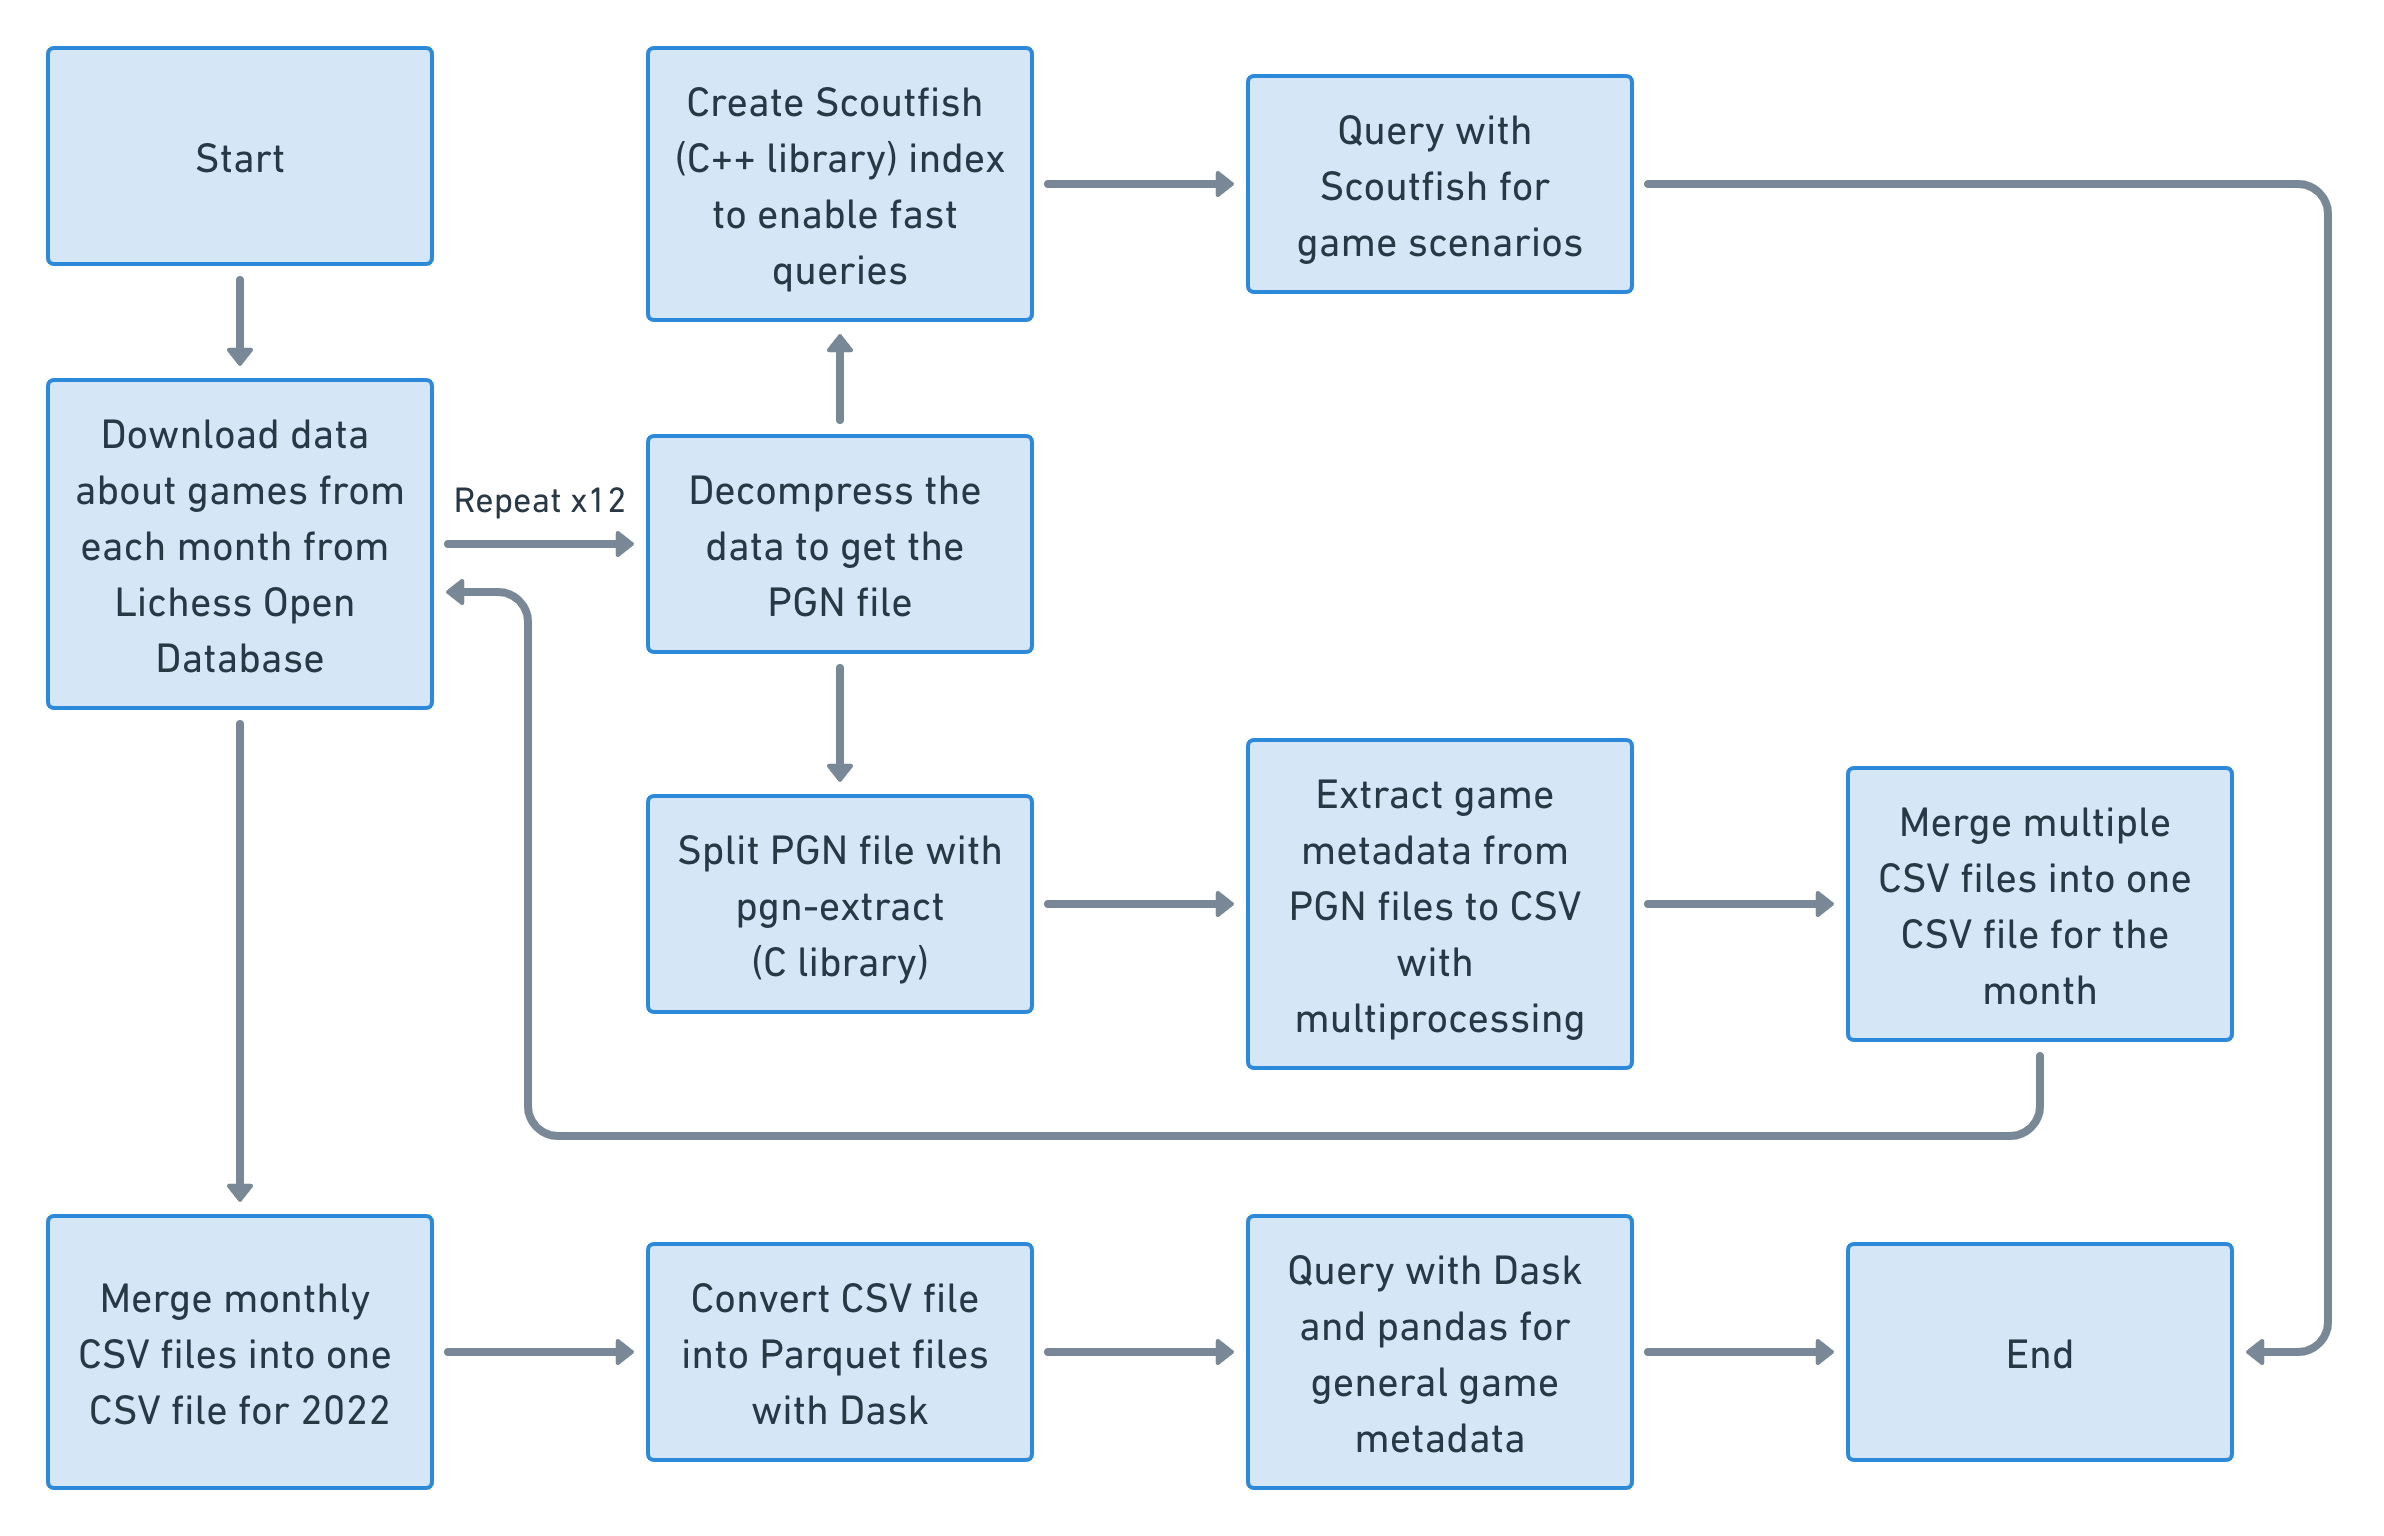
\includegraphics[width=0.8\textwidth]{Data Pipeline.png}
\end{figure}

Figure \ref{fig:dataPipeline} shows an overview of our data pipeline. It shows how we used the Lichess Open Database to collect the data over 12 months. To analyse game metadata, we aggregated the data into a single CSV file, and converted it to a folder of Parquet files to query with Dask.

We also created a Python script to convert the CSV file to an SQLite3 database -- this enables us to perform queries on the data over SQL for manual data exploration, which is easier and more interactive than using Dask functions.

\subsection{Subsampling for Machine Learning Models}
Machine learning is computationally expensive, so generating and testing machine learning models in a reasonable amount of time would be infeasible. Therefore, we will further subsample the data. We will use a random sample of 12.5\% of the original sample size, which is approximately 5 million games. Since we are not trying to predict rare events and we are still using a large sample, our subsampling should have minimal impact on the representativeness of our insights -- patterns that we identify for 5 million games should also be present in the complete data set.

\section{Project Results and Evaluation}
In this section, we will start by exploring the data to understand the data set better before implementing machine learning models to uncover patterns in how people play chess. We will explain our motive and the development of each machine-learning model before discussing the results and evaluating their insights.

\subsection{Data Exploration}

\subsubsection{Structure of Data}
Our data consists of 40,121,728 Rated Blitz and Rated Rapid games that were played on Lichess in 2022. Each game is described by: the datetime of when the game started, what type of game (Rated Blitz or Rapid) it was, the specific time control, outcome of the game (1-0 for a White win, 1/2-1/2 for a draw, and 0-1 for a Black win), how the game ended, ECO category of the opening, the specific opening that was played, who played White and Black, their Lichess ratings, and a URL to the game on Lichess. Figure \ref{fig:structureOfData} shows the head of the DataFrame, which contains the first two games in the data sample -- note that this has been transposed to maintain readability.

\begin{figure}[H]
    \centering
    \caption{Structure of Data}
    \label{fig:structureOfData}
    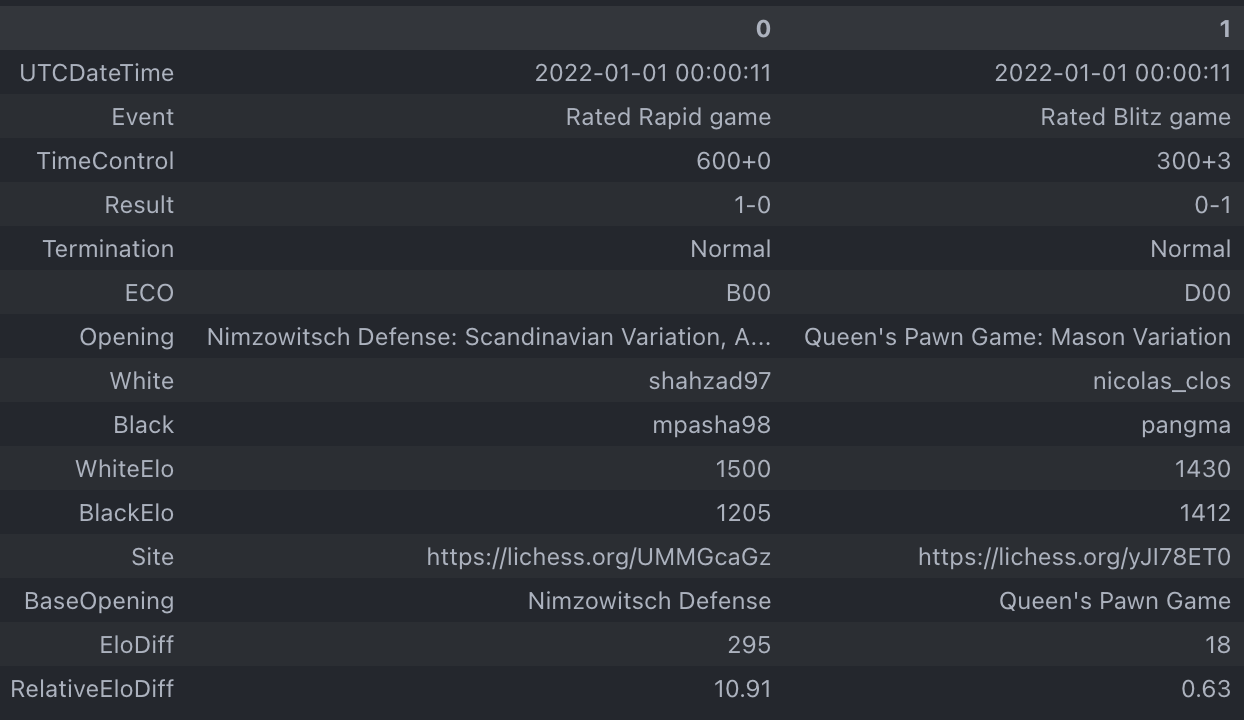
\includegraphics[width=0.6\textwidth]{Structure of Data Transposed.png}
\end{figure}

\subsubsection{Distribution of Player Ratings}
We counted the ratings of players in our data set. Rating systems are designed to predict the outcome of games so that players can be matched fairly. There are various rating systems used in chess -- the most common is the Elo rating system, which is used by various sports. Lichess uses the Glicko 2 rating system, which accounts for volatility amongst other factors to provide better prediction accuracy than the Glicko 1 and Elo rating systems \cite{chessRatingSystems, DeloitteFIDEChessRatingChallenge}. The Glicko 2 rating system starts at 1500, and it is artificially limited to a minimum of 600 in Lichess. We created bins of 200 rating point groups starting from 600 -- this handles the representation of new players well, as those who have played few games will not have changed their rating significantly and likely get placed in the 1400-1600 bin. Note that the last four bins on the right of the bar chart do exist, but they are difficult to see -- they contain totals of 11,622 for 2800-3000, 382 for 3000-3200, 459 for 3200-3400, and 1 player for 3400-3600. In addition, the counts are based on each game played, so some players may be overrepresented in the data set -- a player who plays 100 games within the year will have 100 entries in the data set, whereas a player who plays 1 game will have 1 entry. However, this is not a significant issue because the data set is large enough to represent the distribution of player ratings well.

Figure \ref{fig:distributionOfPlayerRatings} shows that the distribution of player ratings tends towards a normal distribution. We could explain this based on the concept that a player's performance is similar to a random walk, which states that an object moves randomly with equal probability in different directions. In Lichess ratings, a player's rating can be seen as the result of a series of random walks, where the player's rating constantly changes as they win and lose games. Over time, their rating will tend to stabilise to represent their true skill level. Moreover, the central limit theorem states that the sum of a large number of independent and identically distributed random variables tends towards a normal distribution \cite{le1986central}. In this case, the ratings of individual players can be seen as independent and identically distributed random variables, with each game representing a single trial. Therefore, the central limit theorem predicts that the distribution of ratings will tend towards a normal distribution as the number of games increases. This is supported by how largest bin is the 1400-1600 bin, which contains the starting rating of 1500. Lichess' matchmaking system could contribute to this -- it matches players with similar skill, so games theoretically end up with a roughly equal number of wins and losses.

\begin{figure}[H]
    \centering
    \caption{Distribution of Player Ratings on Lichess in 2022}
    \label{fig:distributionOfPlayerRatings}
    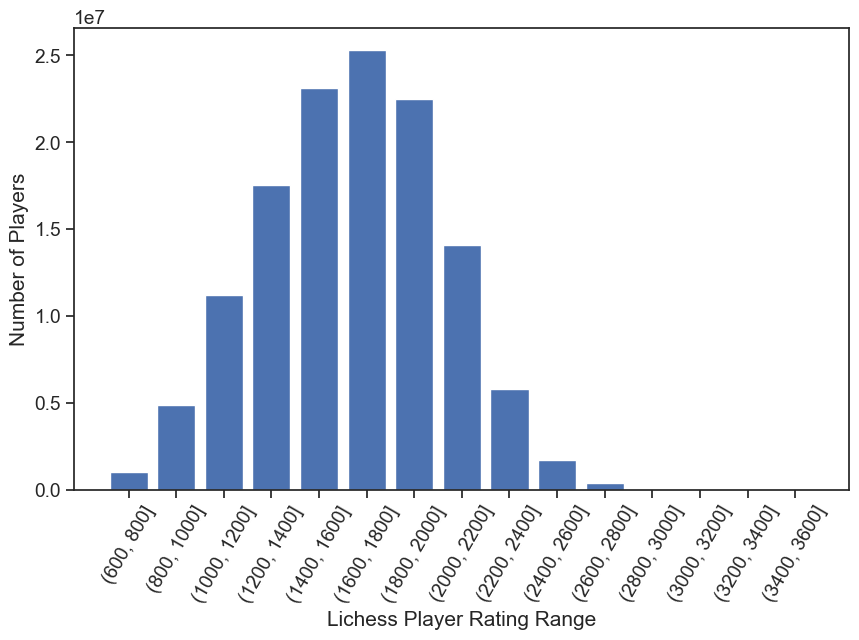
\includegraphics[width=0.8\textwidth]{Distribution of Player Ratings.png}
\end{figure}

\subsubsection{Effect of Rating Difference on Win Rate}

\begin{figure}[H]
    \centering
    \caption{Mean White Win Rate for Each RelativeEloDiff Bin}
    \label{fig:meanWhiteWinRateForEachRelativeEloDiffBin}
    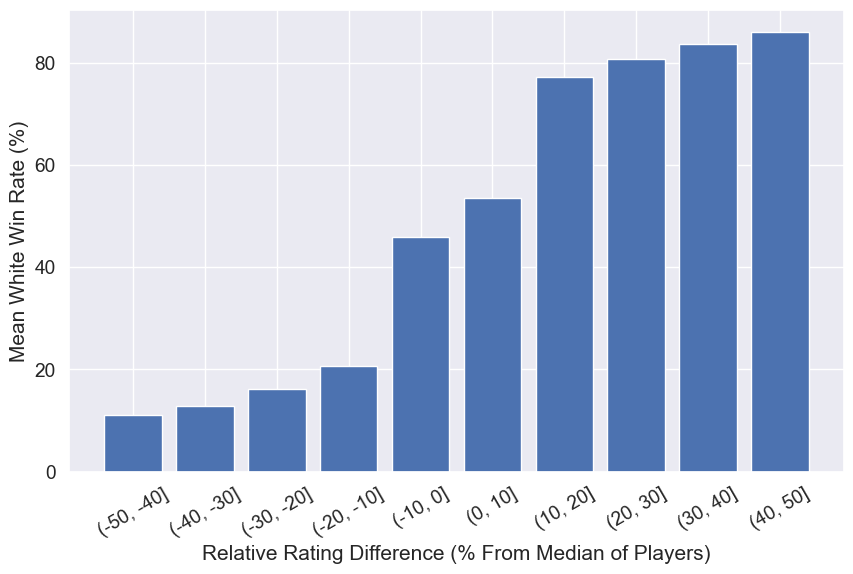
\includegraphics[width=0.8\textwidth]{Mean White Win Rate for Each RelativeEloDiff Bin.png}
\end{figure}

Next, we investigated the impact of player rating differences on White's win rate. To begin with, we counted the outcomes of all games, and then counted the outcomes of games when White had a higher rating -- White won 49.69\% of all games, which rose to 53.98\% of games when they had a higher rating than their opponent (as shown in figure \ref{fig:effectOfHigherRatingOnWhiteWinRate} from the appendices). Then, we sought to quantify the impact of rating difference in both absolute and relative terms -- the former was the difference in rating between the two players, and the latter was the difference in rating divided by the mean rating of the two players. Figure \ref{fig:distributionOfAbsoluteRatingDifference} and figure \ref{fig:distributionOfRelativeRatingDifference} from the appendices show the distribution of the absolute and relative rating differences. We grouped the data by rating difference and calculated the win rate for White. For example, when White is rated 1100 and Black is rated 900, the absolute rating difference is 200, whereas the relative rating difference is 10\%. We focused on the win rate for White because the opening of the game is usually decided by White.

The results showed that there is a clear positive correlation between rating difference and White's win rate. Both the absolute and relative difference metrics corroborate this, but we saw that relative rating difference highlighted the impact of rating on White's win rate more clearly. Absolute rating difference (shown in figure \ref{fig:meanWhiteWinRateForEachEloDiffBin} from the appendices) is more intuitive to understand, but it is less accurate than relative rating difference (shown in figure \ref{fig:meanWhiteWinRateForEachRelativeEloDiffBin}) because it is not normalised.

\subsubsection{Most Popular Openings by Category}

We also counted the most popular openings by category in figure \ref{fig:mostPopularOpeningsByCategory}, as this is represented by the ECO column provided in the Lichess PGN data. ECO (Encyclopedia of Chess Openings) is a classification of chess openings based on the first few moves of the game. Editors who mostly consist of chess grandmasters select critical opening lines and assign them a code \cite{matanovic1971classification}. The ECO system consists of five categories, A to E, each of which represent a category of opening. Within each category, there are further subcategories to group openings more explicitly. For example, a game with an ECO code of A41 means that the opening is a flank opening as it is in the A category, and the 41 means that the opening was the Queen's Pawn Game. The ECO system is not perfect as it does not include all openings (as demonstrated by the 32,799 games with the unknown category in figure \ref{fig:mostPopularOpeningsByCategory}), but it is useful to analyse opening trends.

\begin{figure}[H]
    \centering
    \caption{Most Popular Openings by Category on Lichess in 2022}
    \label{fig:mostPopularOpeningsByCategory}
    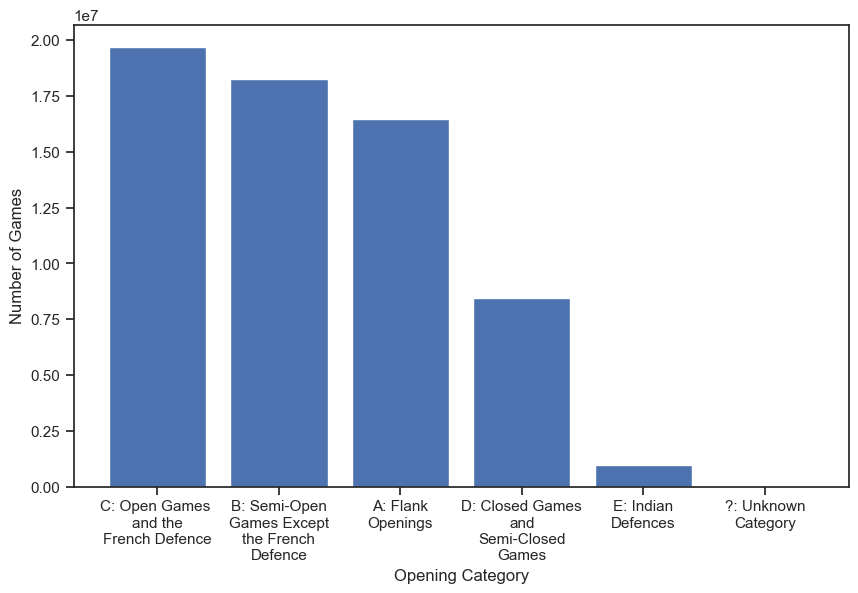
\includegraphics[width=0.8\textwidth]{Most Popular Openings by Category.png}
\end{figure}

Figure \ref{fig:mostPopularOpeningsByCategory} shows that the most popular category of openings are open games and semi-open games, whereas the Indian defences and closed games are the least popular. This makes sense for the general population of games -- the ideas behind these openings are simple and straightforward, as they focus on controlling the centre and developing pieces quickly. However, we see that the pattern is different for players rated 2000 and above -- semi-open games and flank openings are more popular than open games in this category (shown in figure \ref{fig:mostPopularOpeningsByCategoryRated2000Plus} from the appendices). At higher rated games, players often prefer to play more complex and dynamic openings that enable opportunities to create imbalances in the position and therefore gain an advantage at an earlier stage of the game.

\subsubsection{Most Popular Base Openings}

\begin{figure}[H]
    \centering
    \caption{Most Popular Base Openings on Lichess in 2022}
    \label{fig:mostPopularOpenings}
    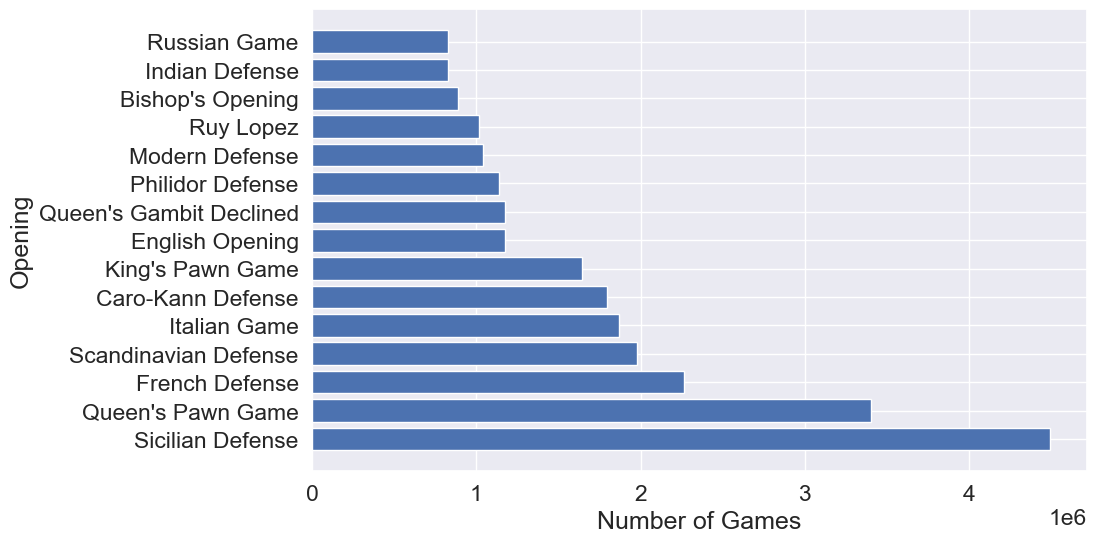
\includegraphics[width=0.8\textwidth]{Most Popular Base Openings.png}
\end{figure}

The data set also includes a column for the specific opening detected in each game based on Lichess' opening detection. We grouped openings that were different variations of each other into base openings to get a more accurate representation -- figure \ref{fig:examplesOfChessOpenings} from the appendices contains examples of base openings on the chess board. The top 15 most popular base openings account for 61.79\% of all games in our data set. Figure \ref{fig:mostPopularOpenings} shows that the most popular openings are the Sicilian Defence and the Queen's Pawn Game by a significant margin. The Sicilian Defence is the most well-studied response to White moving the king's pawn forward by two, which could explain why it is the most popular opening. However, the Queen's Pawn Game is slightly misleading, as it describes any opening beginning with White moving the queen's pawn where they do not play the Queen's Gambit and therefore encompasses a large number of openings such as the London System which are not labelled separately.

Delving deeper into the data, we found that the most popular base openings varied by rating groups. The top players rated 2000 and above strongly preferred the Sicilian Defense compared to other openings (shown in figure \ref{fig:mostPopularOpeningsRated2000Plus} from the appendices). This may be because the Sicilian Defense is a complex opening that requires a lot of preparation due to the number of variations, and it is unanimously accepted as the best response to White opening with the king's pawn. Conversely, the Sicilian Defense becomes much less popular for players rated 1200 and below for the same reasons. Figure \ref{fig:mostPopularOpeningsRated1200Minus} from the appendices shows that the two most popular base openings for this group are the Queen's Pawn Game and the King's Pawn Game, which represent generic openings starting with the queen's pawn and the king's pawn respectively -- this is likely because they are simple and easy for beginners to play.

\subsection{Predicting Game Results Using Classifiers}
We sought to predict the result of a game using classifiers based on some of the features we explored in the previous subsection. Accurate predictions would provide insights into what factors are the most important in determining the outcome of a game -- this could help platforms like Lichess improve their rating system to calculate more appropriate rating changes after each game, thus making the rating system fairer and improving the user experience.

\subsubsection{Implementing the Decision Tree and Random Forest Classifiers}
We used both decision tree classifiers and random forests with various features. Based on the previous section, we focused on features related to player rating and opening. Figure \ref{fig:resultsOfModelsToPredictResultOfAGame} summarises the results we obtained from our models, grouped by type of classifier and sorted by F1 score. We used F1 score as our evaluation metric because it is a good measure of accuracy for imbalanced data sets such as ours, where there are fewer draws compared to wins and losses for White, as it accounts for a balance between precision and recall. We also used accuracy as a secondary metric to compare the performance of our models.

\subsubsection{Results and Evaluating the Decision Tree and Random Forest Classifiers}
In the results table in figure \ref{fig:resultsOfModelsToPredictResultOfAGame}, you can see that we denoted the RelativeEloDiffBin and EloDiffBin features with different increments. We previously binned these features to explore the distribution of values, but we wanted to see whether using finer binning would improve the performance of our models. Hence, we tested the same model but with different binning increments, which we did not include in the table for brevity -- the increments included in the table represent those that produced the best F1 score and accuracy.

\begin{figure}[H]
    \centering
    \caption{Results of Models to Predict the Result of a Game}
    \label{fig:resultsOfModelsToPredictResultOfAGame}
    \begin{tabular}{| l | l | l | l |} 
        \hline
        \bf{Classifier} & \bf{Features} & \bf{F1 Score} & \bf{Accuracy} \\ [0.5ex] 
        \hline
        Decision Tree & BaseOpening, RelativeEloDiffBin (5\% Increments) & 0.510 & 0.521 \\
        \hline
        Decision Tree & ECO, RelativeEloDiffBin (5\% Increments) & 0.508 & 0.521 \\
        \hline
        Decision Tree & BaseOpening, EloDiffBin (10 Increments) & 0.498 & 0.525 \\
        \hline
        Decision Tree & BaseOpening, EloDiff & 0.495 & 0.519 \\
        \hline
        Decision Tree & BaseOpening, RelativeEloDiff & 0.492 & 0.511 \\
        \hline
        Decision Tree & BaseOpening, RelativeEloDiff, TimeControl & 0.486 & 0.496 \\
        \hline
        Decision Tree & BaseOpening, WhiteElo, BlackElo & 0.474 & 0.476 \\ 
        \hline
        Random Forest & BaseOpening, RelativeEloDiffBin (5\% Increments) & 0.509 & 0.521 \\ 
        \hline
        Random Forest & BaseOpening, RelativeEloDiffBin (10\% Increments) & 0.509 & 0.521 \\ 
        \hline
        Random Forest & ECO, RelativeEloDiffBin (5\% Increments) & 0.508 & 0.521 \\ 
        \hline
        Random Forest & BaseOpening, RelativeEloDiff & 0.490 & 0.511 \\ 
        \hline
        Random Forest & BaseOpening, RelativeEloDiff, TimeControl & 0.484 & 0.497 \\ 
        \hline
    \end{tabular}
\end{figure}

There was little difference in the performance of our decision tree classifiers and our random forest classifiers -- both of them achieved similar F1 scores and accuracy when using the same features. However, we saw some variation in performance when using different features. We saw an improvement by binning the RelativeEloDiff values instead of using the raw values -- this is likely because it helps to smooth the noise of tiny differences and help extract the general information that varying RelativeEloDiff provides. Using 5\% increments was the sweet spot between binning too finely and thus introducing noise, and binning too broadly and losing the value of information. Meanwhile, using ECO values rather than BaseOpening values resulted in worse performance, likely due to the ECO categories being too vague, with openings in the same category being vastly different in some cases.

While there are some differences in results between the variations of our models, our classification models generally produced poor F1 scores and accuracy. The best F1 score was 0.510 while the best accuracy was 0.525 -- this indicates that our features were not good predictors of the result of a game. Lichess' matchmaking system pairs opponents of similar skill levels. Thus, the difference in rating between players is often minimal, resulting in a small sample size for the bins representing larger rating differences, which may have contributed to the poor performance. Furthermore, the outcome of a chess game is highly dependent on how the players perform in the game, which is subject to variation, especially in lower-rated games due to human nature -- these are not features that we have in our data set, nor are they features that we can feasibly obtain. Our results show that it is difficult to predict the outcome of a game using the additional features that we explored, and that the rating system used by platforms like Lichess is a good predictor -- we do not have any evidence to suggest how it can be improved.

\subsection{Investigating the Relationship Between Base Opening Popularity and Game Results Using Linear Regression}
Next, we investigated the relationship between the popularity of a base opening and their game results. Our initial hypothesis is that the higher the win rate for White for a base oepning, the more popular it will be -- this is because the opening is mostly decided by White, and they want to maximise their chances of winning. Identifying clear trends could form the foundation for future investigations into how social learning theory can be applied to chess openings and how much other people's preferences affect our own when we play chess.

\subsubsection{Implementing the Linear Regression Models}
We analysed this relationship using a linear regression model to find the relationship between the popularity of a base opening and each game result (White win, Black win, or draw) -- the popularity of a base opening was the independent variable, and the game result was the dependent variable. The models were trained on the subsample of approximately 5 million games, from which we included base openings with more than 10,000 games. When we later filtered the data to investigate trends for high, middle, and low rated players, we included base openings with more than 1,000 games. To evaluate the models, we used the R\textsuperscript{2} score, which is the proportion of the variance in the dependent variable that is predictable from the independent variable. The R\textsuperscript{2} score ranges from 0 to 1 -- an R\textsuperscript{2} score of 1 means that the model explains all the variability in the dependent variable, while an R\textsuperscript{2} score of 0 means that the model explains none of the variability. We also used the mean absolute error, which is the average absolute difference between the predicted and actual values -- the lower the mean absolute error, the better the fit. We chose the mean absolute error over the more common mean squared error because it is more robust to outliers, which is important as we can later evaluate outliers qualitatively within the context of the game.

\subsubsection{Results and Evaluating the Linear Regression Model for All Players}
Figure \ref{fig:popularityOfBaseOpeningVsWinRatesAllPlayers} shows the linear regression for White and Black win rates across all games within our subsample. Our model in figure \ref{fig:popularityOfBaseOpeningVsWhiteWinRateAllPlayers} has an R\textsuperscript{2} score of 0.00476 and a mean absolute error of 59245.291, while our model in figure \ref{fig:popularityOfBaseOpeningVsBlackWinRateAllPlayers} has an R\textsuperscript{2} score of 0.00434 and a mean absolute error of 59350.082. There are some notable outliers in the plot; for example, the top-left point of figure \ref{fig:popularityOfBaseOpeningVsWhiteWinRateAllPlayers} represents the Sicilian Defense. This has many variations and is considered to be the best reply to openings starting with the White king's pawn on e4, but unlike most other openings, it is decided by Black's moves. Thus, it is not surprising that it has a relatively low win rate for White yet is still very popular. The same explanation applies to other defensive openings such as the French Defense, which is also a very popular opening despite having a relatively low win rate for White.

The plots and the metrics both show that the popularity of a base opening has a very weak relationship with the win rate for White and Black. This suggests that players choose to play openings based on more complex factors than just the win rates, such as the difficulty, the length, and the number of variations of the opening. Intuitively, this makes sense -- in the case that every player picked the opening with the highest win rate, it could cause an equilibrium where the win rate for each opening ends up being the same, thus making the strategy ineffective.

\begin{figure}[H]
    \centering
    \caption{Popularity of Base Opening vs. Win Rates (All Players)}
    \label{fig:popularityOfBaseOpeningVsWinRatesAllPlayers}
    \begin{subfigure}{0.49\textwidth}
        \centering
        \caption{Popularity of Base Opening vs. White Win Rate}
        \label{fig:popularityOfBaseOpeningVsWhiteWinRateAllPlayers}
        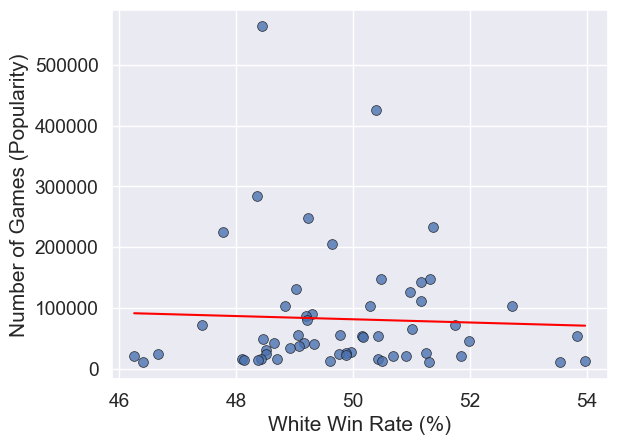
\includegraphics[width=\textwidth]{Popularity of Base Opening vs. White Win Rate (All Rated Players).png}
    \end{subfigure}
    \hfill
    \begin{subfigure}{0.49\textwidth}
        \centering
        \caption{Popularity of Base Opening vs. Black Win Rate}
        \label{fig:popularityOfBaseOpeningVsBlackWinRateAllPlayers}
        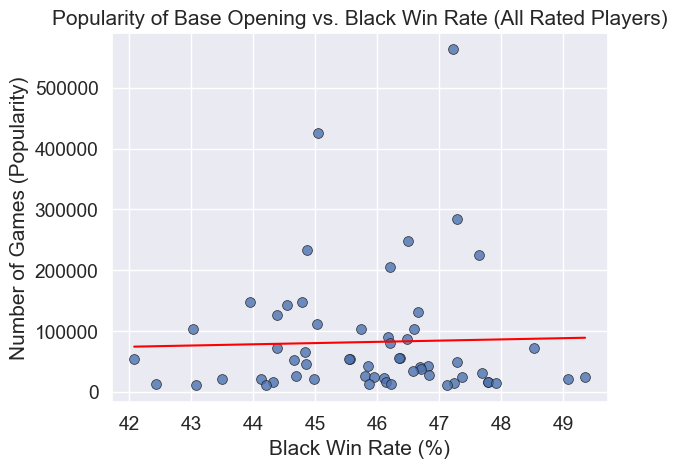
\includegraphics[width=\textwidth]{Popularity of Base Opening vs. Black Win Rate (All Rated Players).png}
    \end{subfigure}
\end{figure}

\subsubsection{Results and Evaluating the Linear Regression Models for Different Rating Groups}
We also generated linear regression models for each rating group and compared their R\textsuperscript{2} scores and mean absolute errors, as shown in figure \ref{fig:metricsForLinearRegressionModelsOfPopularityOfBaseOpeningVsGameResults}. When we generated the linear regression models for each rating group, we found that there were similarly bad metrics for the high and mid rating groups. However, we noticed that at the low rating group, the R\textsuperscript{2} scores and mean absolute errors were significantly better.

\begin{figure}[H]
    \centering
    \caption{Metrics for Linear Regression Models of Popularity of Base Opening vs. Game Results}
    \label{fig:metricsForLinearRegressionModelsOfPopularityOfBaseOpeningVsGameResults}
    \begin{tabular}{| l | l | l | l |} 
        \hline
        \bf{Rating Group} & \bf{Game Result} & \bf{R\textsuperscript{2} Score} & \bf{Mean Absolute Error} \\ [0.5ex] 
        \hline
        High (2000+) & White Win & 0.000233 & 10014.448 \\
        \hline
        High (2000+) & Black Win & 0.00219 & 9964.941 \\
        \hline
        High (2000+) & Draw & 0.00296 & 9959.435 \\
        \hline
        Mid (1201-1999) & White Win & 0.00236 & 34197.744 \\
        \hline
        Mid (1201-1999) & Black Win & 0.00113 & 34230.073 \\
        \hline
        Mid (1201-1999) & Draw & 0.0158 & 33360.013 \\
        \hline
        Low (1200-) & White Win & 0.0451 & 6668.558 \\
        \hline
        Low (1200-) & Black Win & 0.0367 & 6722.418 \\
        \hline
        Low (1200-) & Draw & 0.0260 & 6793.426 \\
        \hline
    \end{tabular}
\end{figure}

Figure \ref{fig:popularityOfBaseOpeningVsWinRatesLowRatedPlayers} shows the linear regression for White and Black win rates across games where White was rated 1200 or below. It is clear that there are stronger positive and negative correlation between White and Black win rate and the number of games played for each base opening. There is a notable change in the x-axes here that shows a broader range of win rates for White and Black -- this makes sense, as newer players tend to be more willing to try different strategies.

Although our linear regression models were not successful in isolation, comparing the results of the models for different rating groups provided insight into the role of social learning in the game of chess. While the fitness of the linear regression models is still not great, it is better than the models for other rating groups, which suggests that there is a greater element of social learning in the low rating group. As lower rated players typically have less experience, they may not have strong preferences for the type of openings they play, and thus may be more likely to follow the trends of other players according to the general win rates of each opening.

\begin{figure}[H]
    \centering
    \caption{Popularity of Base Opening vs. Win Rates (Players Rated 1200 and Below)}
    \label{fig:popularityOfBaseOpeningVsWinRatesLowRatedPlayers}
    \begin{subfigure}{0.49\textwidth}
        \centering
        \caption{Popularity of Base Opening vs. White Win Rate}
        \label{fig:popularityOfBaseOpeningVsWhiteWinRateLowRatedPlayers}
        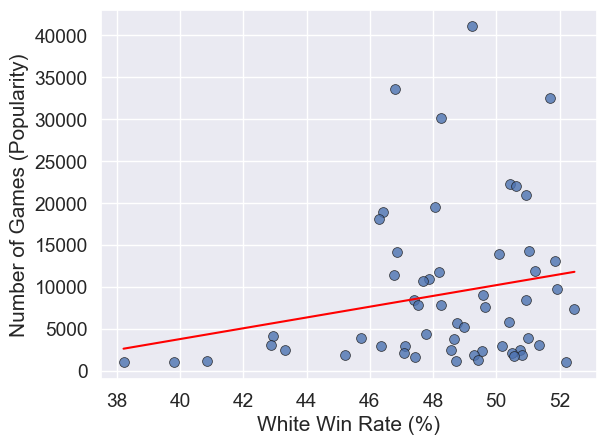
\includegraphics[width=\textwidth]{Popularity of Base Opening vs. White Win Rate (Rated 1200-).png}
    \end{subfigure}
    \hfill
    \begin{subfigure}{0.49\textwidth}
        \centering
        \caption{Popularity of Base Opening vs. Black Win Rate}
        \label{fig:popularityOfBaseOpeningVsBlackWinRateLowRatedPlayers}
        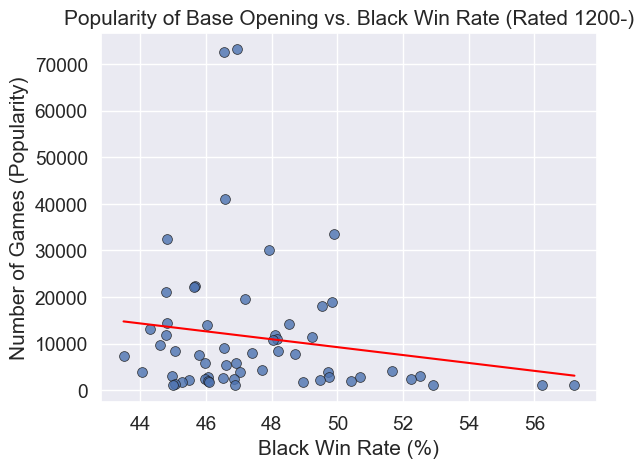
\includegraphics[width=\textwidth]{Popularity of Base Opening vs. Black Win Rate (Rated 1200-).png}
    \end{subfigure}
\end{figure}

\subsection{Clustering Base Openings by Game Results}
Following our earlier exploration of the most popular base openings, we investigated whether we could cluster them by game results. Accurate clusters would allow us to identify base openings that are more likely to result in a certain outcome -- this could be useful in determining someone's style of play, thus opening the possibility for more fine-tuned analysis of match-ups between players.

\subsubsection{Calculating Proportion of Game Results Per Base Opening}

\begin{figure}[H]
    \centering
    \caption{Proportion of Game Results for the Top 15 Most Played Base Openings}
    \label{fig:proportionOfGameResultsForTop15BaseOpenings}
    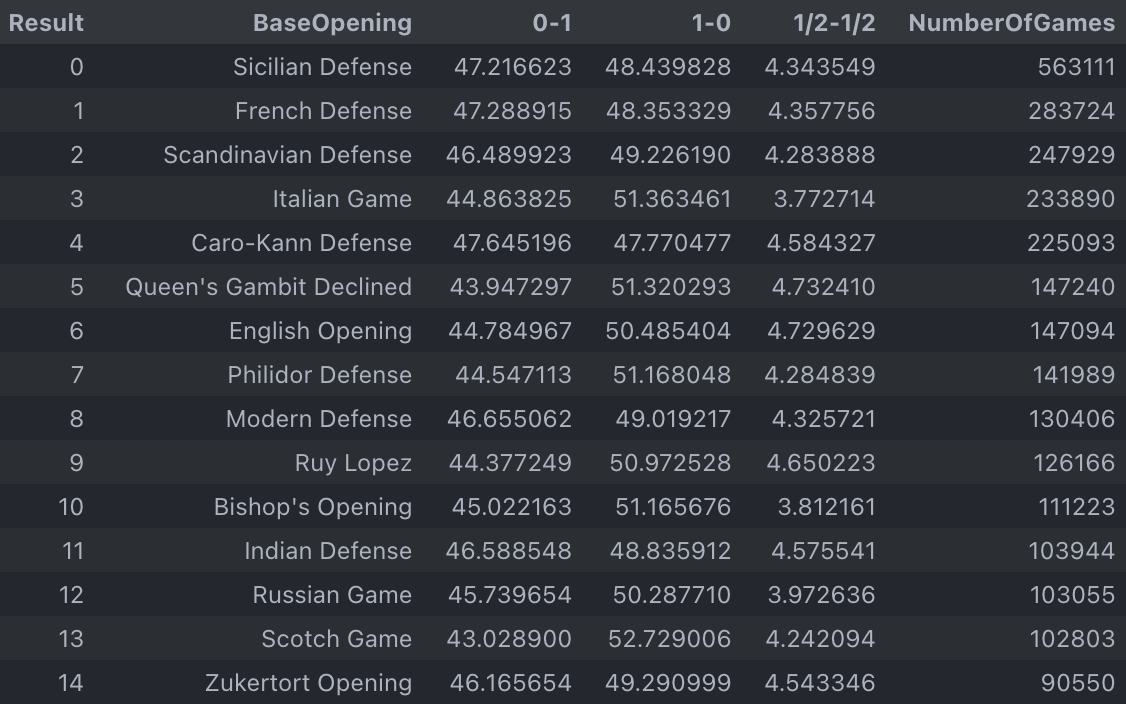
\includegraphics[width=0.8\textwidth]{Proportion of Game Results for Top 15 Base Openings.png}
\end{figure}

Before applying our clustering algorithm, we needed to aggregate the data to obtain the proportion of game results per base openings. This involved counting the number of outcomes for each base opening, and then calculating the proportions of each outcome. Note that we filtered the data to only include base openings with a significant sample size to remove outliers and thus improve the quality of our clustering. We required a minimum of 10,000 games, which was reasonable for the subsample of approximately 5 million games. Furthermore, we filtered out the King's Pawn Game and the Queen's Pawn Game, as these openings are too generic and would add unwanted noise. Figure \ref{fig:proportionOfGameResultsForTop15BaseOpenings} shows the proportion of game results for the top 15 base openings, sorted in descending order of the number of games.

\subsubsection{Implementing K-Means Clustering}
We decided to use K-means clustering over alternatives such as hierarchical agglomerative clustering because it is easy to implement and interpret, and our underlying data is relatively simple. We used the percentages of each game result for our features and we used the elbow method to determine the optimal number of clusters. The elbow method involves plotting the explained variation (also known as the within-cluster sum of squares -- WCSS) as a function of the number of clusters, and then choosing the number of clusters at the elbow of the curve. Figure \ref{fig:elbowMethodForBaseOpeningsClusteredByGameResults} shows the elbow method for our data -- we can see that the elbow occurs at four clusters.

\begin{figure}[H]
    \centering
    \caption{Elbow Method for K-Means Clustering of Base Openings by Game Results}
    \label{fig:elbowMethodForBaseOpeningsClusteredByGameResults}
    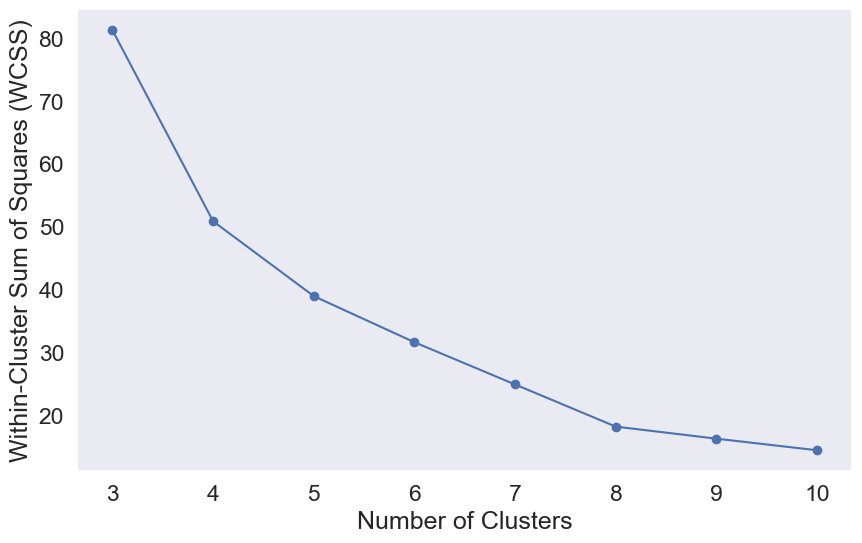
\includegraphics[width=0.6\textwidth]{Elbow Method for Clustering of Base Opening by Results.png}
\end{figure}

Additionally, we recorded the silhouette score for each number of clusters to validate our choice. The silhouette score is a measure of how similar an object is to its own cluster compared to other clusters -- it ranges from -1.0 to 1.0, where a higher score is good and indicates that the object is well-matched to its own cluster and poorly-matched to neighbouring clusters. Figure \ref{fig:silhouetteScoresForBaseOpeningsClusteredByGameResults} shows the silhouette score for each number of clusters from 3 to 10 -- it confirms that the optimal number of clusters is four, with the best silhouette score of 0.478.

\begin{figure}[H]
    \centering
    \caption{Silhouette Scores for K-Means Clustering of Base Openings by Game Results}
    \label{fig:silhouetteScoresForBaseOpeningsClusteredByGameResults}
    \begin{tabular}{| l | l |} 
        \hline
        \bf{Number of Clusters} & \bf{Silhouette Score} \\ [0.5ex] 
        \hline
        3 & 0.444 \\
        \hline
        4 & 0.479 \\
        \hline
        5 & 0.459 \\
        \hline
        6 & 0.448 \\
        \hline
        7 & 0.449 \\
        \hline
        8 & 0.451 \\
        \hline
        9 & 0.468 \\
        \hline
        10 & 0.426 \\
        \hline
    \end{tabular}
\end{figure}

\subsubsection{Results and Evaluating the Clusters}
Figure \ref{fig:baseOpeningsClusteredByGameResultsWhiteVersusBlack} shows how our method clustered the base openings relative to the win rate for White and Black. It has a silhouette score of 0.479 and a within-cluster sum of squares of 50.827. Note that the axes for the win rates of either side are different, yet this is appropriate because White is generally expected to win more games than Black due to first mover advantage. We can see that the four clusters are fairly distinct, with the middle two clusters being the most distinct. Cluster 1 contains openings that were highly successful for Black -- they resulted in a win rate that was similar to White's win rate. Conversely, cluster 2 contains openings that were highly successful to White, with a much greater delta between White's win rate and Black's win rate than expected. Clusters 3 and 0 are less distinct, but we can see that cluster 3 shows openings with a slight advantage for Black, while cluster 0 shows openings with a slight advantage for White.

\begin{figure}[H]
    \centering
    \caption{Base Openings K-Means Clustered by Game Results}
    \begin{subfigure}{0.49\textwidth}
        \centering
        \caption{White Win Rate vs. Black Win Rate}
        \label{fig:baseOpeningsClusteredByGameResultsWhiteVersusBlack}
        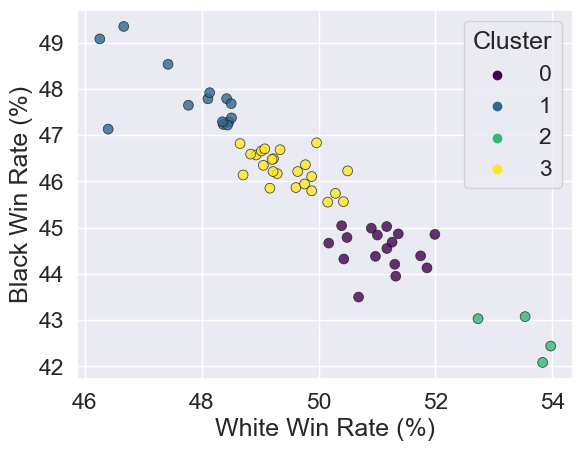
\includegraphics[width=\textwidth]{Base Openings Clustered by Game Results (White Win Rate vs Black Win Rate).png}
    \end{subfigure}
    \hfill
    \begin{subfigure}{0.49\textwidth}
        \centering
        \caption{White Win Rate vs. Draw Rate}
        \label{fig:baseOpeningsClusteredByGameResultsWhiteVersusDraw}
        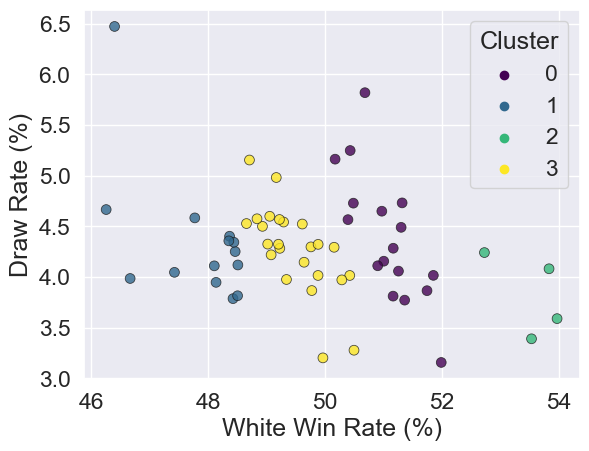
\includegraphics[width=\textwidth]{Base Openings Clustered by Game Results (White Win Rate vs Draw Rate).png}
    \end{subfigure}
\end{figure}

Meanwhile, figure \ref{fig:baseOpeningsClusteredByGameResultsWhiteVersusDraw} shows the clustering based on the win rate for White against the draw rate. It highlights the limitations of our clustering algorithm -- the clusters in this figure are much less distinct compared to the previous figure, with some slight overlap between the clusters. The draw rate does not appear to have much of an effect on the clusters -- this is likely because the draw rate is relatively low, which leaves little room for variation, and thus the effect is not strong enough to be picked up by our clustering algorithm.

Overall, our clustering algorithm was successful in differentiating between the base openings based on whether White or Black won. Our clusters may be used in analysing the opening preferences of players -- lower rated players who play openings that are highly successful for White may need to reconsider the understanding of the openings they play, as they may be losing games despite having a slight advantage in theory. On the other hand, higher rated players who play openings that are theoretically less successful for White could be investigated further, as it indicates that they may be playing these openings in a different way to make them more successful than expected.

However, our clustering algorithm was unsuccessful in differentiating between the base openings based on draw rate -- this could be improved in the future using a different feature set, such as the number of moves played in each game. If we were able to generate better clusters for draw rate, we could use this to analyse whether players prefer to play more aggressive games that are more likely to end in a win, or more passive games that are more likely to end in a draw. Online platforms like Lichess could account for this in their matchmaking system to ensure that players are matched with opponents of varying play styles to make player ratings more accurate over time.

\subsection{Clustering Base Openings by the Mean Difference of Game Results in Variations}
Our final investigation sought to cluster base openings by the mean difference of the game results between their variations. For example, the Sicilian Defense famously has a number of variations, including the Najdorf Variation, the Dragon Variation, and the French Variation. Our initial hypothesis is that base openings will have varying degrees of difference in outcomes between their variations -- more passive openings such as the Indian Defense will have little difference because their moves depend less on their opponent, whereas more aggressive openings such as the King's Gambit Accepted will have bigger differences due to a more open centre and thus a greater number of viable moves. Accurate clusters would provide a way to quantify how passive or aggressive a base opening is, whereas the chess community traditionally relies on intuition and experience to make these assessments qualitatively.

\subsubsection{Calculating the Mean Difference of Game Results in Opening Variations}

\begin{figure}[H]
    \centering
    \caption{Examples of Euclidean Distances for Opening Variations}
    \label{fig:euclideanDistancesForOpeningVariations}
    \begin{subfigure}{0.49\textwidth}
        \centering
        \caption{Euclidean Distances for Russian Game Variations}
        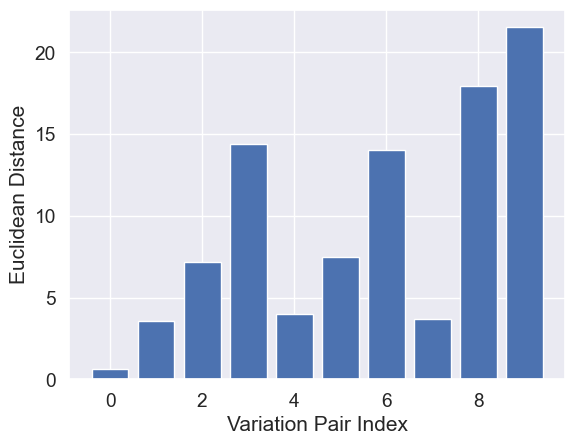
\includegraphics[width=\textwidth]{Euclidean Distances for Russian Game.png}
    \end{subfigure}
    \hfill
    \begin{subfigure}{0.49\textwidth}
        \centering
        \caption{Euclidean Distances for Slav Defense Variations}
        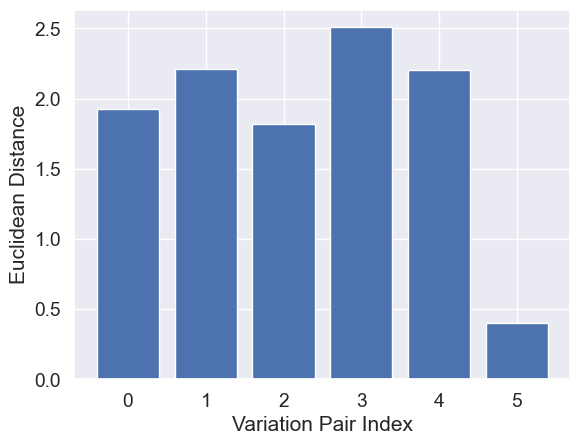
\includegraphics[width=\textwidth]{Euclidean Distances for Slav Defense.png}
    \end{subfigure}
\end{figure}

Similar to previous analyses, we calculated the proportion of game results, but we split this by opening variation. Once we had this data, we filtered it to only include variations that had over 5,000 games to ensure that variations were representative of the base opening -- this reduced the data to 182 variations amongst 32 base openings. Based on this, we used the Euclidean distance formula to quantify the difference between the game results of each variation. Figure \ref{fig:euclideanDistancesForOpeningVariations} shows examples of the Euclidean distances for the Russian Game and the Slav Defense openings. We then calculated the mean difference of the game results between each variation of a base opening. Figure \ref{fig:top15BiggestAndSmallestMeanDifferenceOfBaseOpenings} shows the top 10 base openings that showed the biggest and smallest differences in their variations. There are signs in figure \ref{fig:top15BiggestMeanDifferenceOfBaseOpenings} that our hypothesis about more aggressive openings like the King's Gambit Accepted having bigger differences being true, and likewise for the Sicilian Defense in figure \ref{fig:top15SmallestMeanDifferenceOfBaseOpenings}.

\begin{figure}[H]
    \centering
    \caption{Top 10 Openings with the Biggest and Smallest Differences of Results in Variations}
    \label{fig:top15BiggestAndSmallestMeanDifferenceOfBaseOpenings}
    \begin{subfigure}{0.49\textwidth}
        \centering
        \caption{Biggest Differences of Results in Variations}
        \label{fig:top15BiggestMeanDifferenceOfBaseOpenings}
        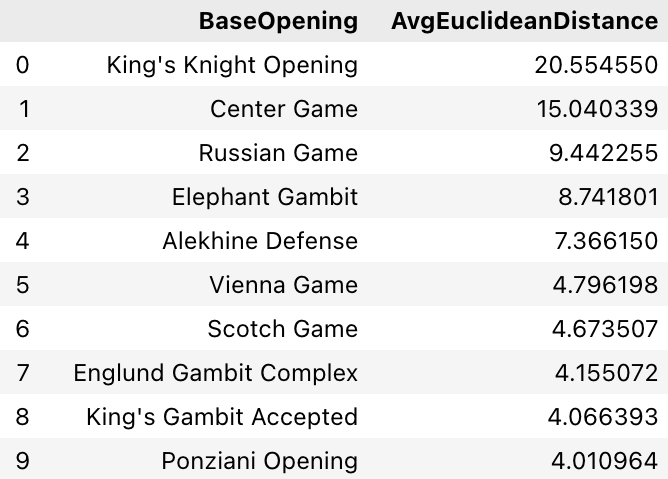
\includegraphics[width=\textwidth]{Top 10 Openings with Biggest Mean Difference in Variations.png}
    \end{subfigure}
    \hfill
    \begin{subfigure}{0.49\textwidth}
        \centering
        \caption{Smallest Differences of Results in Variations}
        \label{fig:top15SmallestMeanDifferenceOfBaseOpenings}
        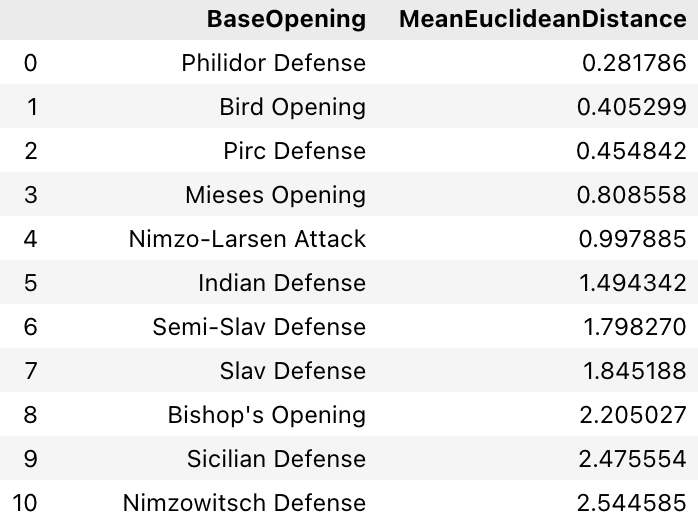
\includegraphics[width=\textwidth]{Top 10 Openings with Smallest Mean Difference in Variations.png}
    \end{subfigure}
\end{figure}

\subsubsection{Implementing K-Means Clustering}
We implemented k-means clustering to see if we could find meaningful clusters based on the mean difference of game results in variations -- this method was the most appropriate for our data because we wanted easily interpretable clusters. We used the elbow method to determine the number of clusters -- figure \ref{fig:elbowMethodForBaseOpeningsClusteredByDifferenceInVariations} suggests that the elbow occurs with four clusters, which suggests that this is the optimal number of clusters.

\begin{figure}[H]
    \centering
    \caption{Elbow Method for K-Means Clustering of Base Openings by the Mean Difference of Results in Variations}
    \label{fig:elbowMethodForBaseOpeningsClusteredByDifferenceInVariations}
    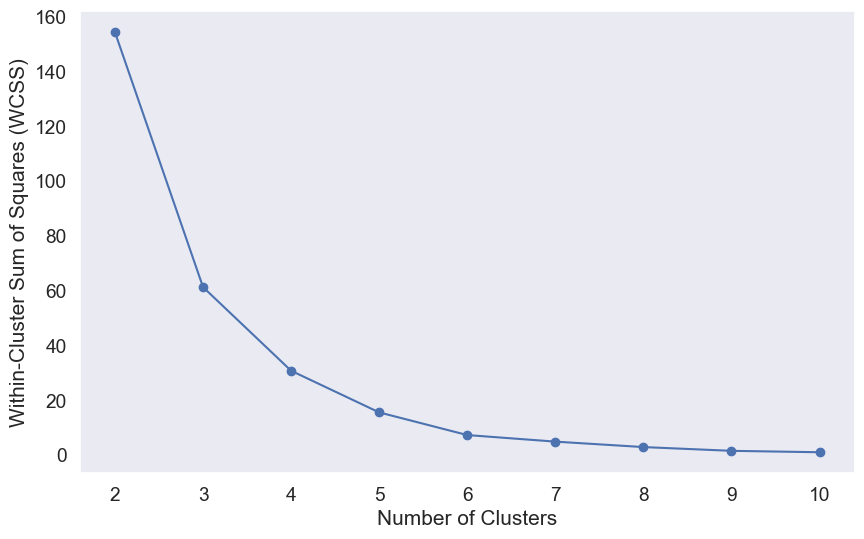
\includegraphics[width=0.8\textwidth]{Elbow Method for Clustering of Base Opening by Difference in Variations.png}
\end{figure}

Furthermore, we used the silhouette method to evaluate the quality of our clusters. Figure \ref{fig:silhouetteScoresForBaseOpeningsClusteredByDifferenceInVariations} shows that the best silhouette score of 0.810 is achieved with two clusters. However, three clusters achieves a similar silhouette score of 0.712, and both of these scores are significantly higher than the others. Hence, considering the elbow method and the silhouette scores holistically, we decided to use three clusters, as this would provide us with more information than two clusters.

\begin{figure}[H]
    \centering
    \caption{Silhouette Scores for K-Means Clustering of Base Openings by the Mean Difference of Results in Variations}
    \label{fig:silhouetteScoresForBaseOpeningsClusteredByDifferenceInVariations}
    \begin{tabular}{| l | l |} 
        \hline
        \bf{Number of Clusters} & \bf{Silhouette Score} \\ [0.5ex] 
        \hline
        2 & 0.810 \\
        \hline
        3 & 0.712 \\
        \hline
        4 & 0.578 \\
        \hline
        5 & 0.555 \\
        \hline
        6 & 0.578 \\
        \hline
        7 & 0.587 \\
        \hline
        8 & 0.563 \\
        \hline
        9 & 0.603 \\
        \hline
        10 & 0.639 \\
        \hline
    \end{tabular}
\end{figure}

\subsubsection{Results and Evaluating the Clusters}

\begin{figure}[H]
    \centering
    \caption{Base Openings Clustered by the Difference of Results in Variations}
    \label{fig:baseOpeningsClusteredByDifferenceOfResultsInVariations}
    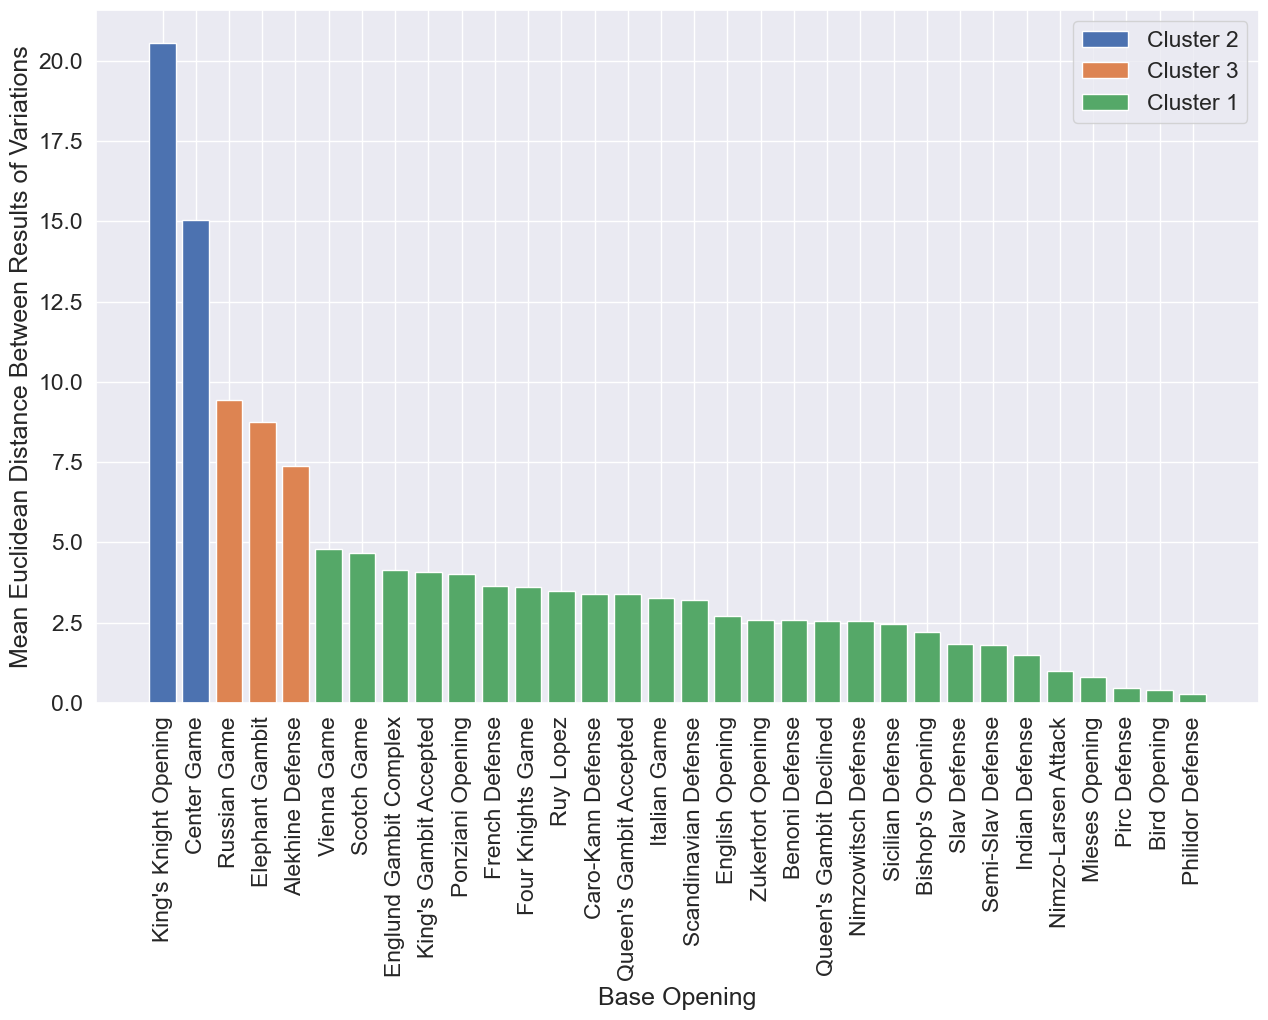
\includegraphics[width=\textwidth]{Base Openings Clustered by Difference in Variations.png}
\end{figure}

Figure \ref{fig:baseOpeningsClusteredByDifferenceOfResultsInVariations} shows our base openings clustered by the difference of results in variations. As shown in the previous sub-subsection, this configuration with three clusters has a within-cluster sum of squares of 61.263 and a silhouette score of 0.712, which indicates that the clusters are compact and well-separated. The quality of our clusters is also backed up visually, as there are three distinct clusters. Cluster 2 contains openings that have a large difference between results of variation, whereas cluster 3 contains openings with a medium difference, and cluster 1 contains openings with a small difference.

We can see that openings in cluster 1 tend to consist of more passive openings and mostly consist of defense openings such as the the Slav Defense. Defensive openings typically follow a set sequence of moves from White and Black as they respond to each other -- these sequences have been well-studied by grandmasters, making players more likely to follow moves by the book and therefore avoid making an early mistake. However, the openings within this cluster vary in passiveness -- the Slav Defense and the Sicilian Defense are in this cluster, yet the Sicilian Defense is considered much more aggressive while the Slav Defense is considered one of the more passive openings in chess \cite{slavDefenseAnalysis}. In cluster 3, it progresses to openings that are slightly more aggressive. For example, it contains the Alekhine Defense, which is also a defense opening, but it is more aggressive than others because it focuses on giving White early control of the centre, encouraging them to overextend so Black can eventually form a counter-attack \cite{alekhinesDefenseAnalysis}. Finally, cluster 2 contains the most aggressive openings. Both of them involve contesting for the centre early on, which leaves both players with more opportunities to make mistakes as a single move could leave either player at a numerical disadvantage in a trade or leave a piece vulnerable to capture. For example, the Center Game involves White moving their king's pawn and their queen's pawn two spaces forward, which enables them to move both bishops freely to form attacks \cite{centerGameAnalysis}.

The clusters support our initial hypothesis suggesting that the more aggressive the opening, the more likely it is that the results will differ. Aggressive openings place more emphasis on the early game, meaning that each move has a greater influence on the balance of the game -- a single mistake could lead to a significant advantage for one player. Thus, it is more likely that the results of variations will differ in aggressive openings, as players are more likely to make mistakes in these openings -- this is supported by the fact that the openings in cluster 2 are the most aggressive, and the openings in cluster 1 are the most passive. Hence, our clustering algorithm was successful -- while it is not a perfect result due to the inconsistency in passiveness of openings in cluster 1, it provides a starting point for quantifying the aggressiveness of openings in the future.

\section{Project Discussion and Conclusion}
In this project, we implemented various machine learning algorithms to analyse chess games, which have provided us with insights into patterns in chess games. We implemented a data pipeline, enabling us to extract data from the Lichess database, transform it into a format suitable for our machine learning algorithms, and load it into Dask and pandas DataFrames. Then, we explored the data and performed feature engineering before implementing classification models, a regression model, and k-means clustering to analyse the data.

\subsection{Project Outcomes}
We created decision tree classifiers and random forest classifiers with various features such as base opening and relative rating difference to predict the result of chess games. Our results found that decision tree classifiers performed equally to random forest classifiers for the features we used, although both of them performed poorly -- the best F1 score was only 0.510. It showed that it is difficult to predict the outcome of a game based on chess game metadata as the patterns in chess games are complex and difficult to capture -- the rating system used by Lichess is therefore a good predictor, as we have no evidence to suggest how it could be improved. Although our models performed poorly, this study was successful in showing us the limitations of our data.

Next, we investigated the relationship between the popularity of base openings and their game results using linear regression, generated for all rated players followed by a separate regression for different rating groups. We found a very weak relationship between the popularity of a base opening and White win rate, with an R\textsuperscript{2} of 0.00476, which suggests that players generally choose to play openings on more complex factors than solely win rate. However, there was a significantly stronger relationship between the two variables for low rated players (1200 and below), with an R\textsuperscript{2} score of 0.0451 between popularity of a base opening and White win rate. Despite all of our linear regression models being unsuccessful in isolation, this study was successful when comparing the rating groups -- it suggests that there is a greater element of social learning in lower rated players, who typically have less experience and are therefore more likely to follow the crowd.

We also performed k-means clustering on base opening to cluster them by their game results. Our clusters based on the win rate for White and Black were successful, as they generated four distinct clusters with a silhouette score of 0.479 and a within-cluster sum of squares of 50.827. Base openings were categorised as being highly successful for White, somewhat successful for White, somewhat successful for Black, or highly successful for Black. The results suggest that higher rated players who play openings that are theoretically less successful for White could be investigated further, as they may be playing these openings in a unique way that makes them more successful at using the opening than the general player base, and it provides a mechanism for easily flagging such players.

Finally, we performed k-means clustering on base openings to cluster them by the mean Euclidean distance of game results in their variations. This study was the most successful, as we generated three distinct clusters with a silhouette score of 0.712 and a within-cluster sum of squares of 61.263. The clusters were categorised as having a small difference between results of variations, a medium difference, or a large difference. Our results suggest that more aggresive base openings are more likely to have a large difference between the results of their variations, providing a mechanism for quantifying the aggressiveness of base openings, which is currently a qualitative and subjective measure.

Overall, the project has been very successful in discovering patterns and insights into how people play chess based on historical data. We have fully fulfilled each of the objectives we set out in the project specification, from creating the data pipeline, to exploring the data and performing feature engineering, to implementing machine learning algorithms and evaluating their usefulness in providing insights into chess games.

\subsection{Limitations}
Despite the success of our project, there were still some limitations. A significant limitation is that it took a long time to collect and process the data -- this prevented us from using move sequence data from the original PGN files. We only used the metadata of games, so we missed out on potentially key information such as the number of blunders made by each player, which could have improved the poor results of our classification models. Our project focused on high-level analysis of games, whereas low-level analysis could have provided different insights. For example, how often do players blunder in different rating groups?

Moreover, we only considered chess games from Lichess, which is a popular online platform for people to play chess, but not the only one. There are other platforms such as Chess.com with large player bases that may have different patterns in how people play chess. We also only considered games from 2022, which restricted us from performing time series analysis on the data.

\subsection{Future Work}
In the future, we could expand our data pipeline to include more data sources, such as the FICS Games Database that we mentioned at the start, to gain access to different metadata. The FICS Games Database records the number of moves in the game, which could be a strong feature to use in our classification models and regression models. Our initial hypothesis is that the number of moves in the game is a strong indicator of the game result, as longer games are more likely to end in a draw due to a lack of material to capture the opponent's king. Using a variety of data sources also allows us to compare the habits of players on different players, which is another avenue for future work.

Additionally, Scoutfish would enable us to perform a low-level analysis of chess games beyond the metadata. For example, it could look at endgame move sequences to determine which endgames are most popular and which subsequences are likely to lead to a win. As endgames are not categorised like openings, this could provide unique insights into the game of chess. The importance of moves in the endgame is also likely to be more influential on the outcome of the game, as there are fewer moves to consider. Thus, it could prove valuable in determining patterns in how people play chess. As it is written in C++, Scoutfish is also more capable of handling larger data sets compared to our data pipeline based on Python. The main problem with Scoutfish is that it is difficult to form queries, but we could have worked around this if we had more time.

We could also use Stockfish to perform a low-level analysis of chess games. Stockfish already identifies moves that were blunders, mistakes or inaccuracies, so we could use this information for future studies. For example, can we predict a player's rating based on how often they blunder? Given the number of blunders made by a player and the average rating of players in a game, can we predict the outcome of the game? These types of questions are more difficult to answer, but they could provide more valuable insights into how people play chess.

Finally, using data from a longer period would allow us to perform time series analysis on the data. We could implement regression models to investigate how the popularity of openings has changed as the number of search results for them on Google Trends has changed over time. As we mentioned at the start, chess is becoming increasingly prevalent in popular cultures, such as with the release of The Queen's Gambit in 2020, so this study would provide us with further insights into how social learning influences how people play chess.

\bibliography{main.bib}
\bibliographystyle{ieeetr.bst}

\newpage
\begin{appendices}

\section{Additional Outputs}
\begin{figure}[H]
    \centering
    \caption{Effect of Higher Rating on White Win Rate on Lichess in 2022}
    \label{fig:effectOfHigherRatingOnWhiteWinRate}
    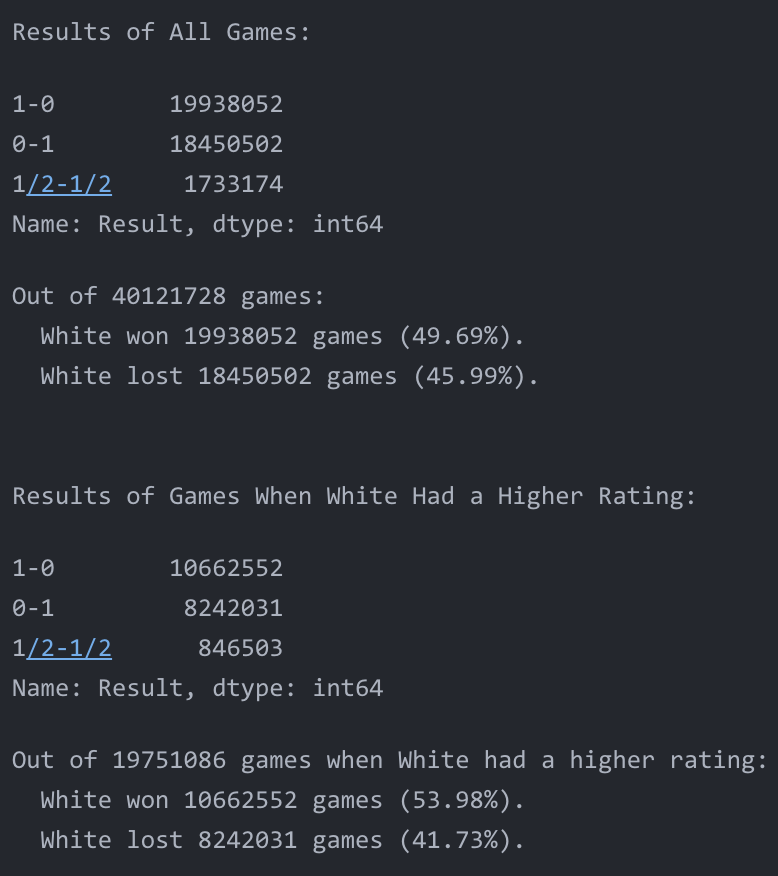
\includegraphics[width=0.5\textwidth]{Effect of Higher Rating on White Win Rate.png}
\end{figure}

\section{Additional Plots}
\begin{figure}[H]
    \centering
    \caption{Distribution of Absolute Rating Difference on Lichess in 2022}
    \label{fig:distributionOfAbsoluteRatingDifference}
    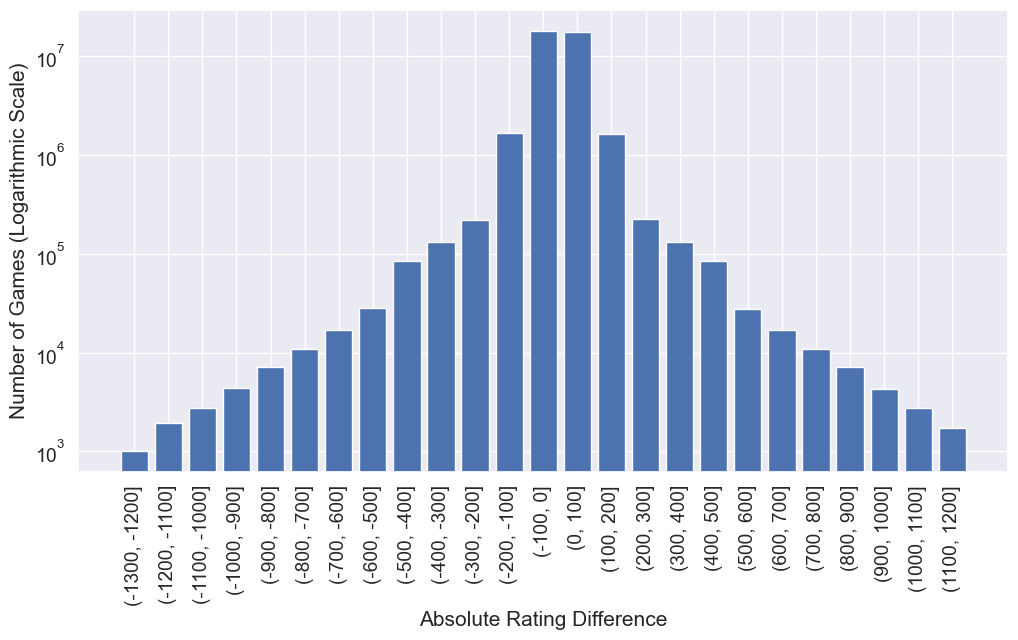
\includegraphics[width=0.8\textwidth]{Distribution of Absolute Rating Difference.png}
\end{figure}

\begin{figure}[H]
    \centering
    \caption{Distribution of Relative Rating Difference on Lichess in 2022}
    \label{fig:distributionOfRelativeRatingDifference}
    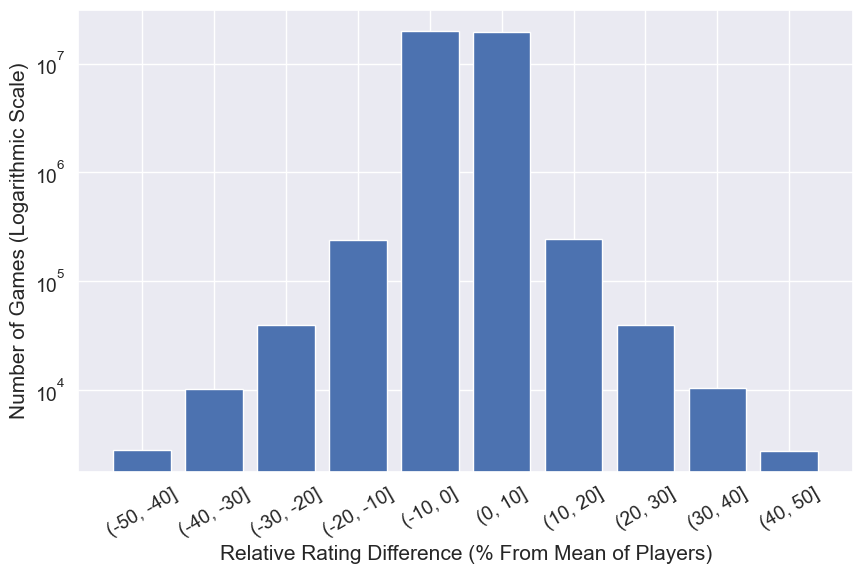
\includegraphics[width=0.8\textwidth]{Distribution of Relative Rating Difference.png}
\end{figure}

\begin{figure}[H]
    \centering
    \caption{Mean White Win Rate for Each EloDiff Bin}
    \label{fig:meanWhiteWinRateForEachEloDiffBin}
    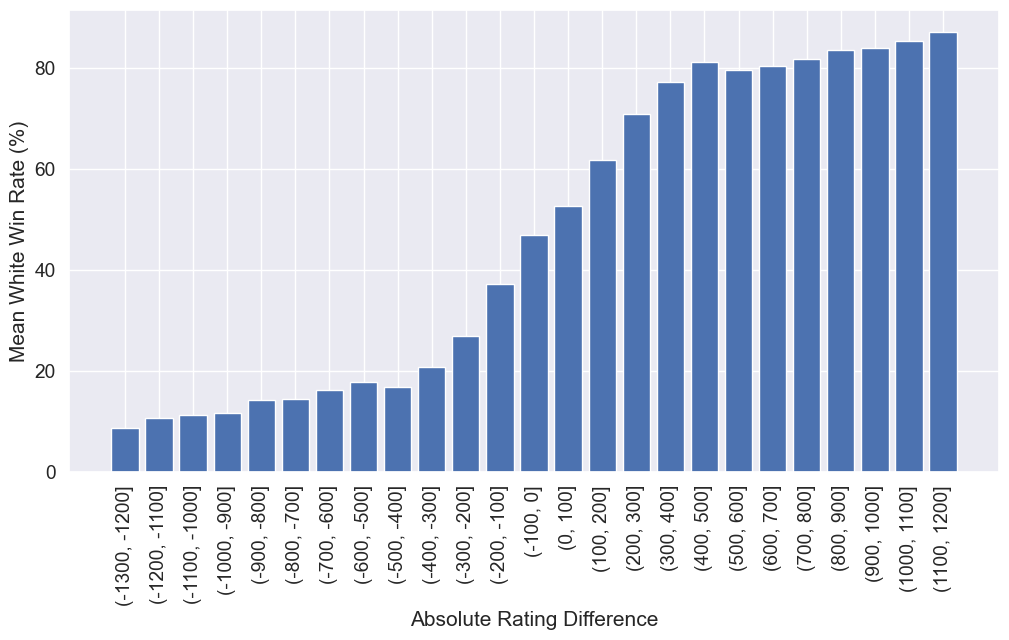
\includegraphics[width=0.8\textwidth]{Mean White Win Rate for Each EloDiff Bin.png}
\end{figure}

\begin{figure}[H]
    \centering
    \caption{Most Popular Openings by Category on Lichess in 2022 (Rated 2000 and Above)}
    \label{fig:mostPopularOpeningsByCategoryRated2000Plus}
    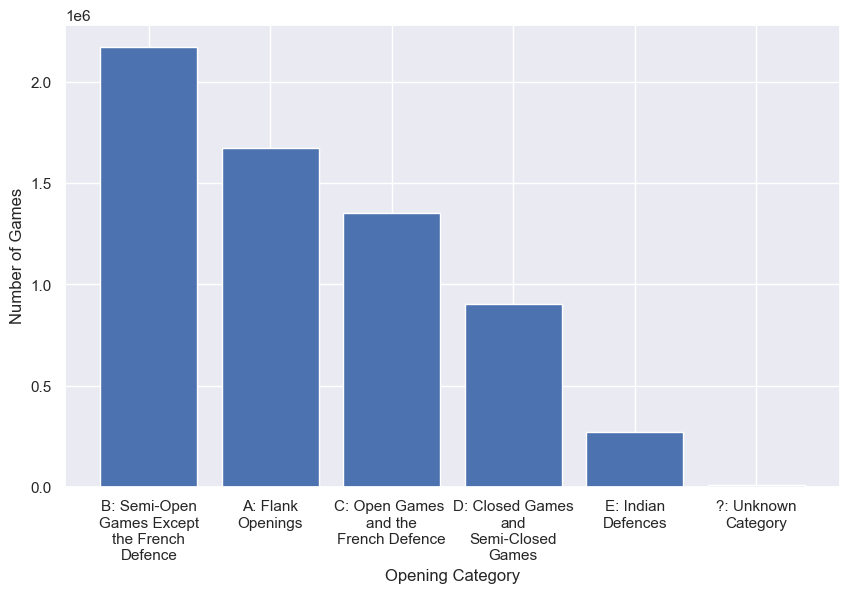
\includegraphics[width=0.8\textwidth]{Most Popular Openings by Category (Rated 2000+).png}
\end{figure}

\begin{figure}[H]
    \centering
    \caption{Most Popular Base Openings on Lichess in 2022 (Rated 2000 and Above)}
    \label{fig:mostPopularOpeningsRated2000Plus}
    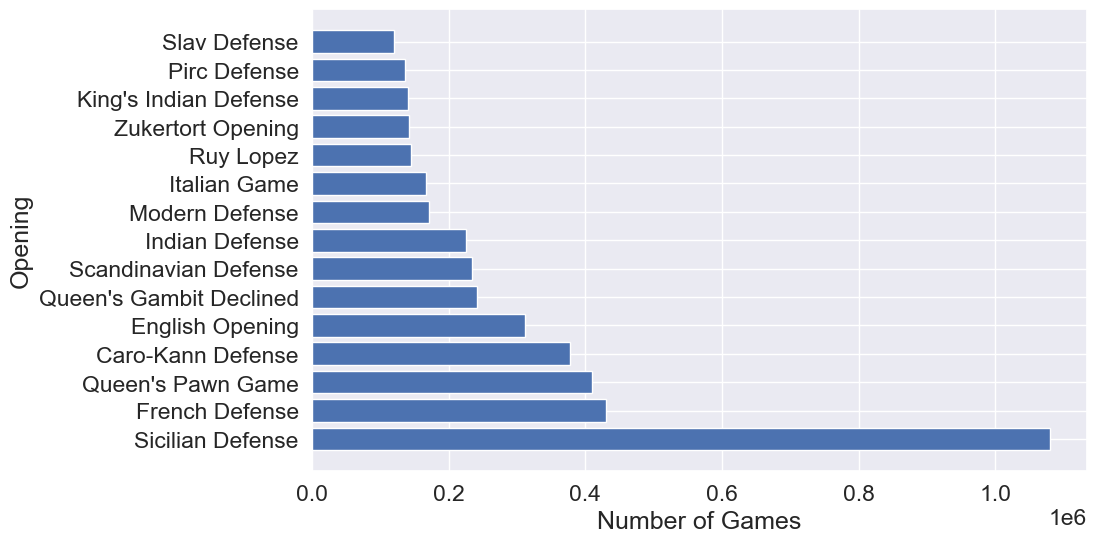
\includegraphics[width=0.8\textwidth]{Most Popular Base Openings (Rated 2000+).png}
\end{figure}

\begin{figure}[H]
    \centering
    \caption{Most Popular Base Openings on Lichess in 2022 (Rated 1200 and Below)}
    \label{fig:mostPopularOpeningsRated1200Minus}
    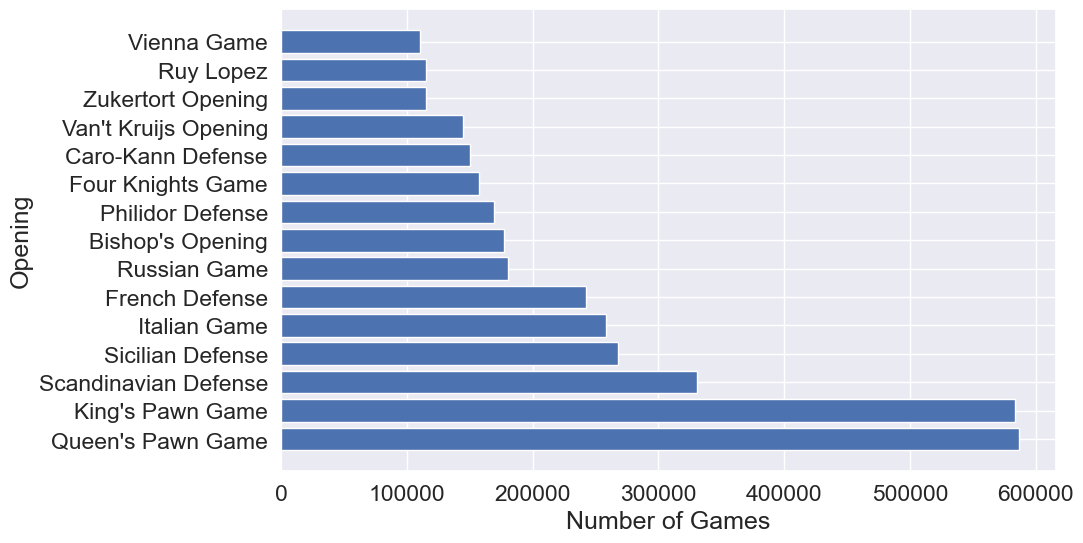
\includegraphics[width=0.8\textwidth]{Most Popular Base Openings (Rated 1200-).png}
\end{figure}

\section{Examples}
\begin{figure}[H]
    \centering
    \caption{Examples of Chess Openings}
    \label{fig:examplesOfChessOpenings}
    \begin{subfigure}{0.49\textwidth}
        \centering
        \caption{Sicilian Defence}
        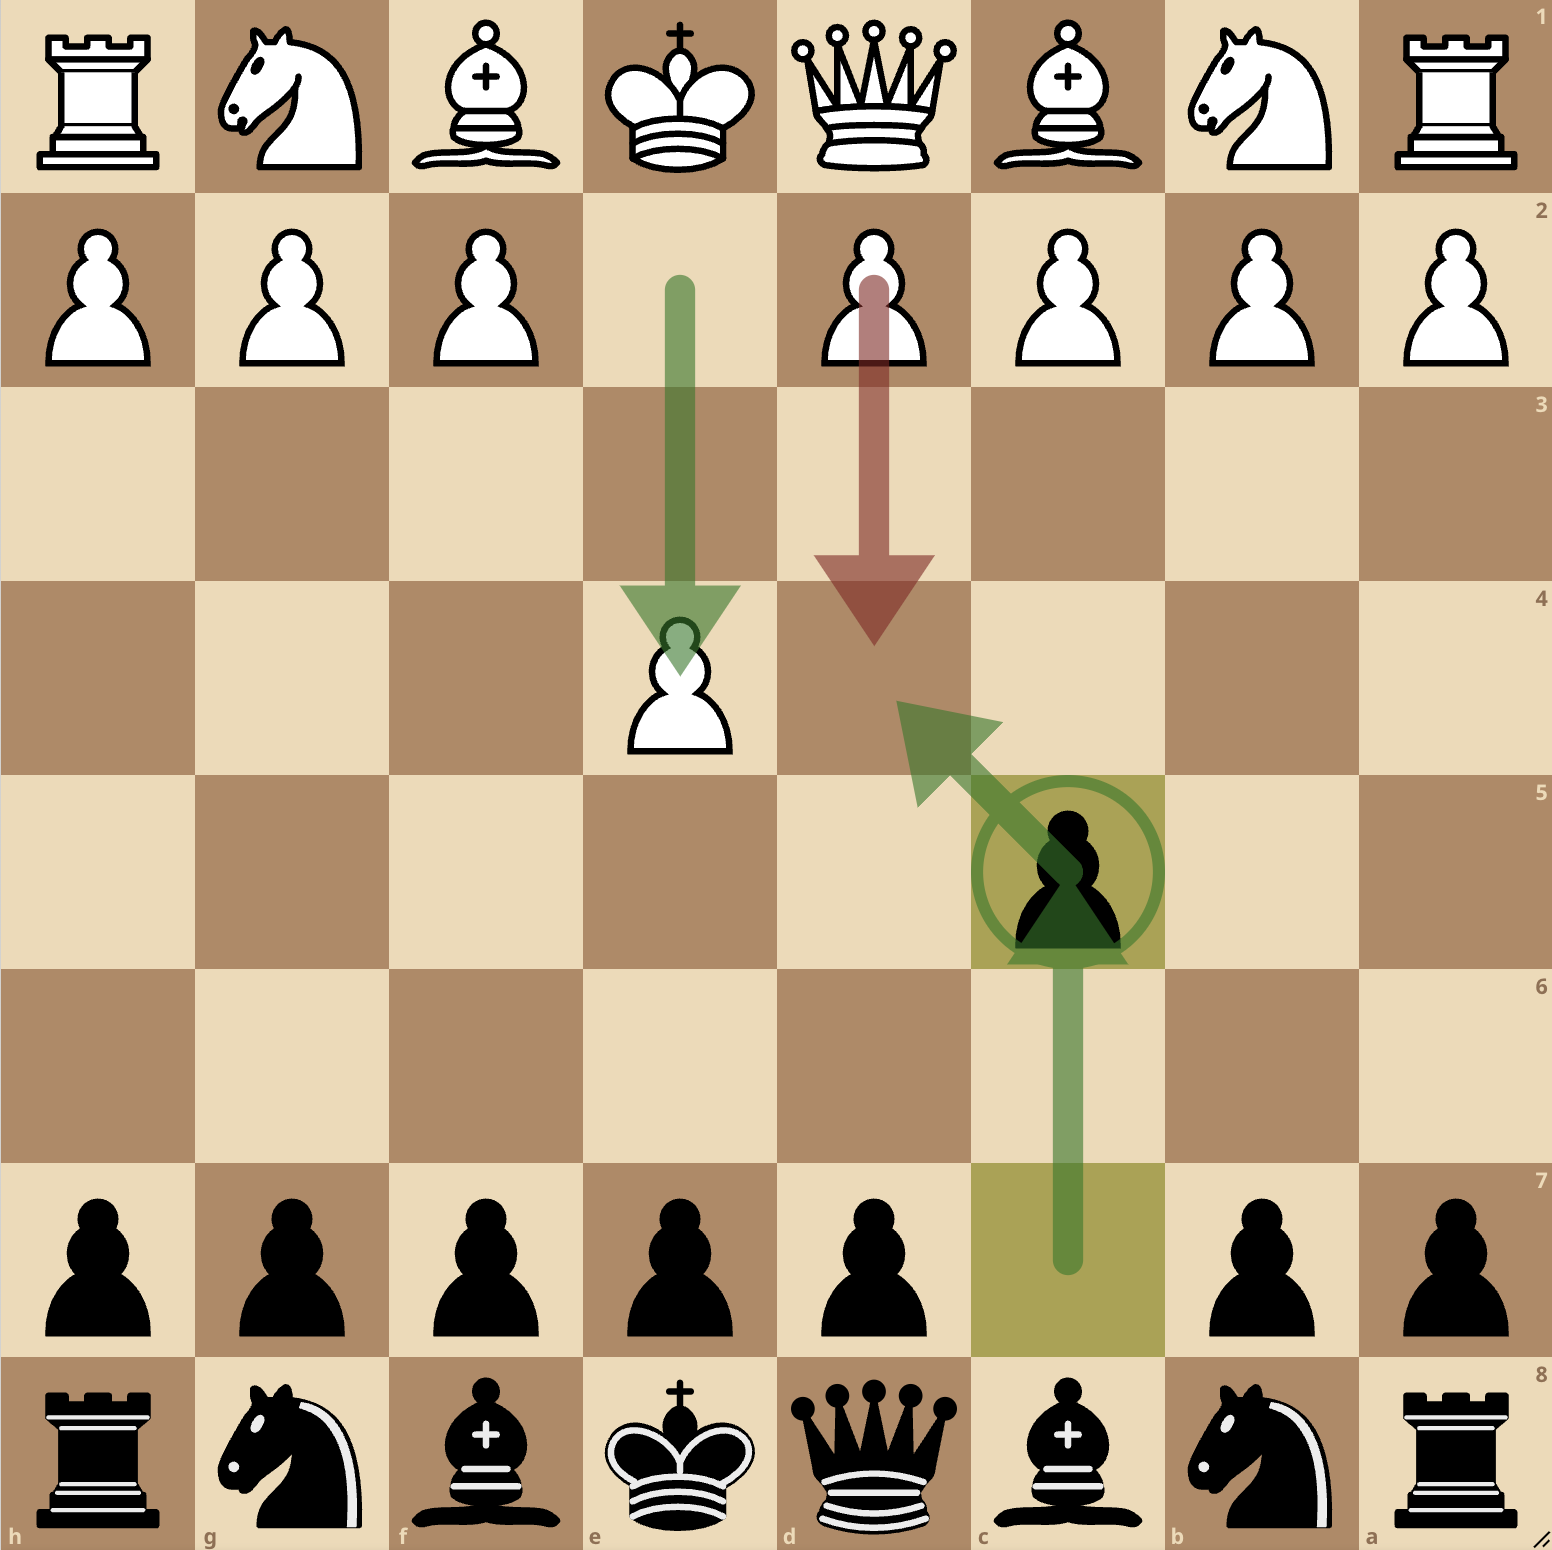
\includegraphics[width=\textwidth]{Example of Sicilian Defence.png}
    \end{subfigure}
    \hfill
    \begin{subfigure}{0.49\textwidth}
        \centering
        \caption{Queen's Gambit}
        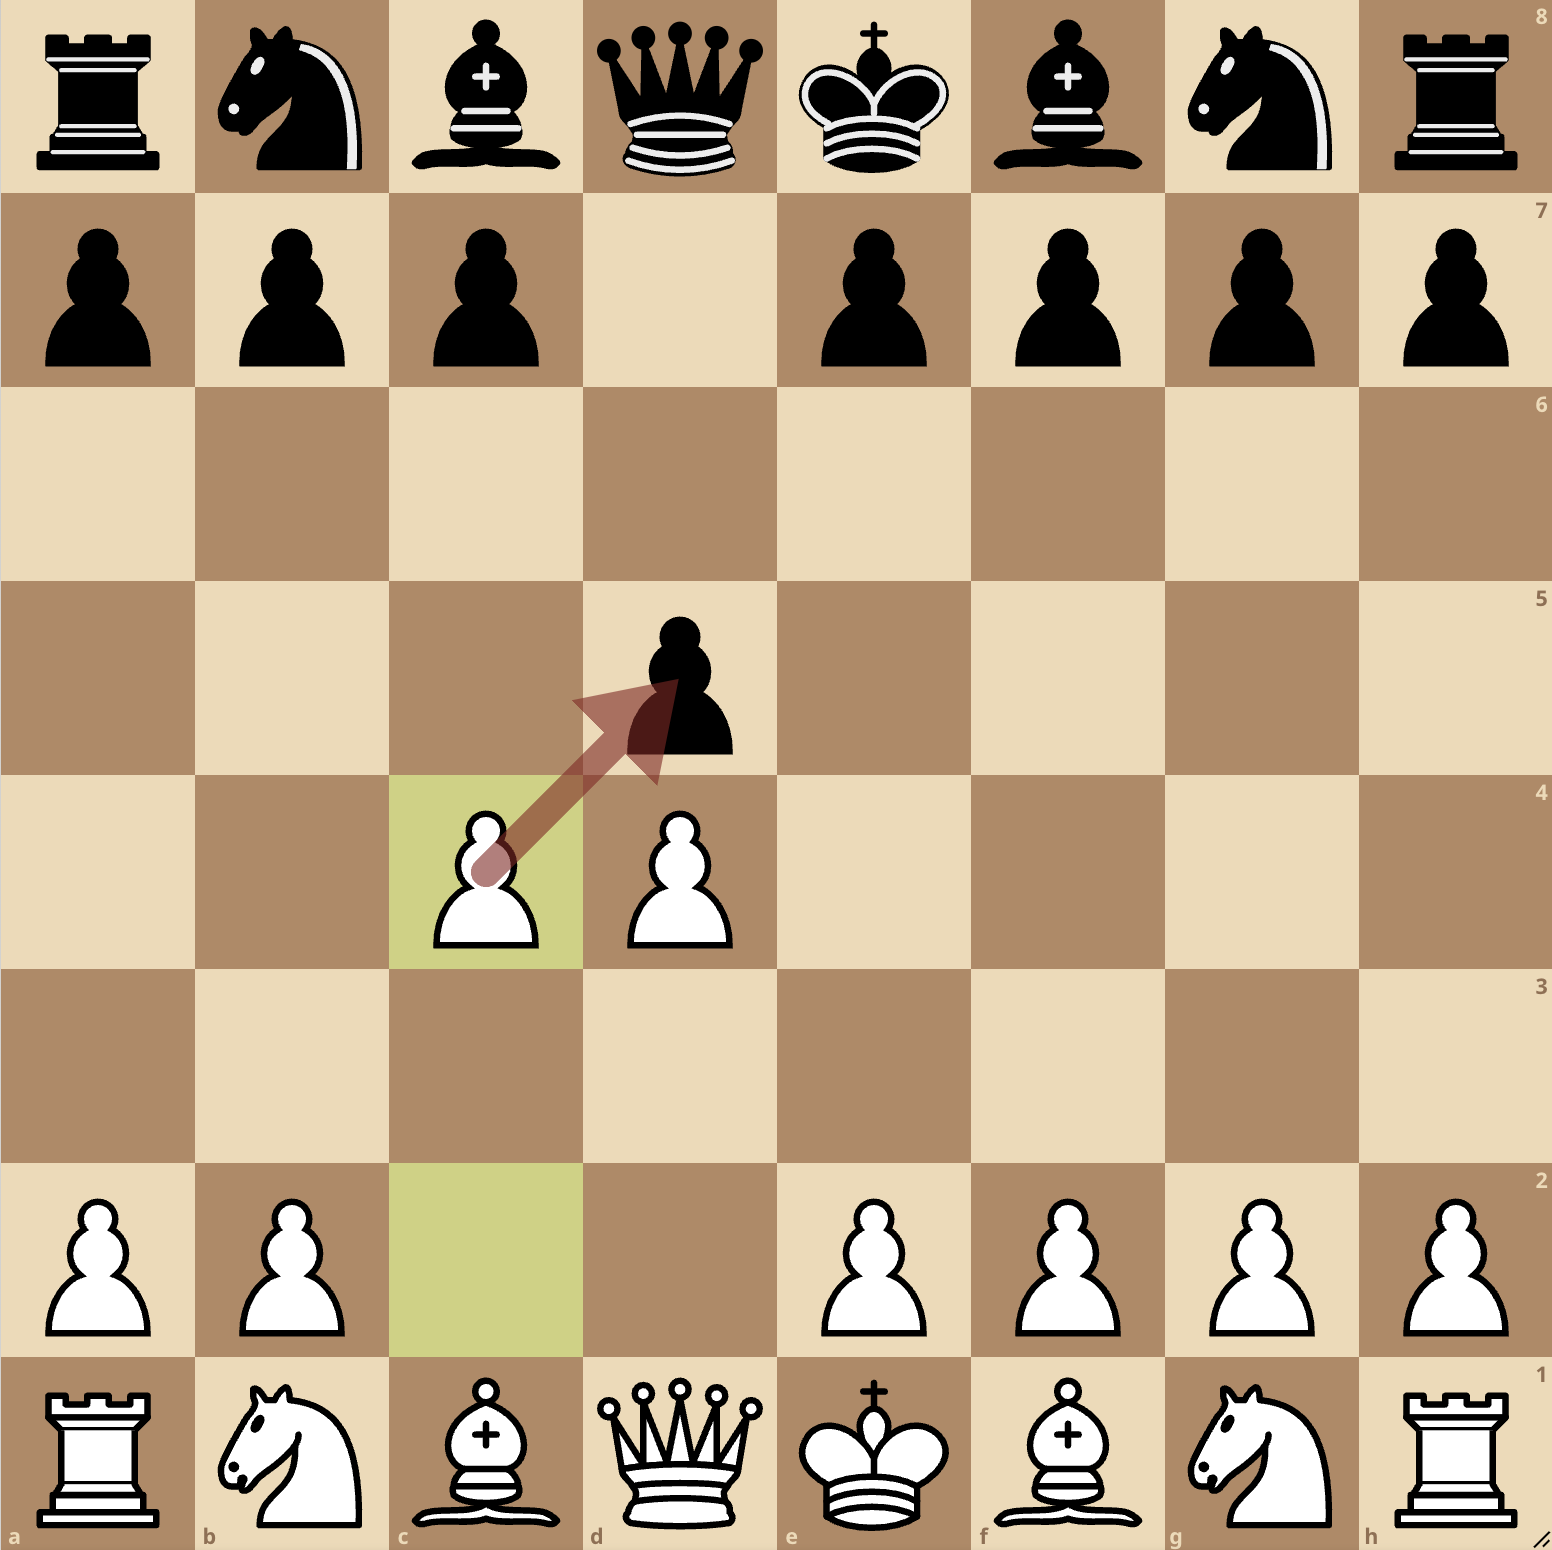
\includegraphics[width=\textwidth]{Example of Queen's Gambit.png}
    \end{subfigure}
\end{figure}

\end{appendices}

\end{document}